% evaluation_tsc.tex -- Section 8 (Experimental Evaluation), journal version, 6-page budget.
% Include from paper.tex with % evaluation_tsc.tex -- Section 8 (Experimental Evaluation), journal version, 6-page budget.
% Include from paper.tex with % evaluation_tsc.tex -- Section 8 (Experimental Evaluation), journal version, 6-page budget.
% Include from paper.tex with % evaluation_tsc.tex -- Section 8 (Experimental Evaluation), journal version, 6-page budget.
% Include from paper.tex with \input{evaluation_tsc/evaluation_tsc}; needs graphicx, booktabs, amsmath, url.
% Generated by paper/package_overleaf.py from paper/sections/evaluation_tsc.tex
% (repository msellamiTN/taas-provenance-discovery, branch research/pamcp-final-evaluation).
\providecommand{\pamcp}{PaMCP}
\section{Experimental Evaluation}
\label{sec:ev}

This section evaluates \pamcp{} against the strongest baselines we could configure. Every result is labelled by
its evidence class: \emph{measured} from the running system, \emph{observed} from executed servers,
\emph{labelled} against reference labels, or \emph{simulated} under stated assumptions; the main comparisons are
confirmed with pre-registered tests.

\subsection{Datasets, Baselines and Evaluation Protocol}
\label{sec:ev-setup}

\begin{table}[t]
\centering
\caption{Datasets and compared methods.}
\label{tab:ev-setup}
\scriptsize
\setlength{\tabcolsep}{2.5pt}
\begin{tabular}{@{}p{2.3cm}p{5.65cm}@{}}
\toprule
\multicolumn{2}{@{}l}{\emph{Data}} \\
Registry & 569 tools, 76 servers (LiveMCPTool \cite{mo2025livemcpbench} + MCPToolBench++ \cite{fan2025mcptoolbench}); 44 annotated \\
Multi-step tasks & 95 LiveMCPBench tasks (test); 60 development prompts \\
Single-tool requests & 60 development / 300 test (50 per category, 66 targets) \\
Calibration suite & 432 items: 6 operations, $n\in\{10,40,160,640\}$, en/fr, noise, context; 264 cal.\ / 168 test \\
Executed servers & 6 MCP reference servers, 37 registry tools \\
Synthetic & cloned and heterogeneous registries ($10^3$--$10^5$); 80 cover and 120 QoS instances \\
\midrule
\multicolumn{2}{@{}l}{\emph{Baselines (adapted to one registry, one encoder; tuned on the development split)}} \\
RAG-MCP \cite{gan2025ragmcp} & dense top-$k$ over the request \\
MCP-Zero \cite{fei2025mcpzero} & model-written requests, server routing \\
COLT \cite{qu2024colt} & collaborative graph of 450 training queries \\
ToolScope \cite{liu2026toolscope} & LLM-confirmed tool merging, subquery retrieval \\
CMTF \cite{suresh2026cmtf} & typed-state search, one tool per step \\
BM25, RRF, per-subtask & lexical, fused, one tool per analyst subgoal \\
\midrule
\multicolumn{2}{@{}l}{\emph{Ablations of \pamcp{}}} \\
G, P, S & gap (Alg.~1), eligibility (Sec.~5), set reasoning + certificate (Sec.~6), $2^3$ design \\
\pamcp{}-L & relevance-first ranking selected on the development split \\
\bottomrule
\end{tabular}
\end{table}

\begin{table}[t]
\centering
\caption{Experimental parameters (defaults in bold).}
\label{tab:ev-params}
\scriptsize
\setlength{\tabcolsep}{2.5pt}
\begin{tabular}{@{}lp{4.3cm}@{}}
\toprule
Parameter & Values \\
\midrule
Profile threshold $\tau$ / risk target & 0.6, 0.75, \textbf{0.9} / 0.05, 0.10 \\
Forging servers $\delta$; false accepts $\varphi$ & 0--0.3 (5 seeds); 0--0.2, \textbf{0.05} \\
Probe coverage $\kappa$; trust $\ell_{\min}$ & 0.25--\textbf{1}; 0.2--0.95, \textbf{0.65} \\
Candidate budget $K$; size matching & 1, 5, \textbf{10}, 20, 40; equal $|K|$ \\
Poisoned descriptions; policies & 10\%, 30\%; least privilege, read-only \\
Registry size; pair relation & 569--$10^5$; eager, partitioned, \textbf{lazy} \\
Cost weights; utility floor $u_{\min}$ & 0, 0.25, \textbf{0.5}, 1; 0--0.9 \\
\bottomrule
\end{tabular}
\end{table}

Table~\ref{tab:ev-setup} lists the data and the compared methods, and Table~\ref{tab:ev-params} the parameters
varied across the experiments. Effects and types are scored against blind labels $J_B$ (Claude Opus), which are
not used to simulate evidence; the simulated verifier uses labels $J_A$ (Claude Sonnet), and we report the
swapped direction and executed servers to remove the dependency between the two. All LLM outputs were recorded
once and are replayed, and every method, including \pamcp{}, was configured on the development split only.
Request-level metrics are resampled with target tools as clusters and task-level metrics with tasks; paired tests
are sign-flip permutation tests, and proportions use Wilson intervals (95\%). Two confirmatory families (F1--F7,
H1--H5) were fixed before the data they test and are Holm-corrected. Code, records, manifests and a notebook that
re-runs every experiment on a CPU are public.\footnote{\url{https://github.com/msellamiTN/taas-provenance-discovery},
branch \texttt{research/pamcp-final-evaluation}; guide in \texttt{docs/REPRODUCIBILITY.md}.}

\subsection{Measured Model Profiles for Model-Conditioned Discovery}
\label{sec:ev-rq1}

The first experiment addresses RQ1, the conditioning of discovery on the deployed model. It tests whether a
measured profile $\rho_{\mathrm{LLM}}$ decides reliably which operations the deployed model keeps, and whether the
gap responds to the model and to the input. Three models answer the calibration suite by reading only, after
stating for each cell their probability of success; $\tau$ is chosen on the calibration split for a risk target
and evaluated on held-out items (measured). The measured profile is compared with two baselines, the model's own
self-assessment and the earlier 64-item profile.

\begin{table}[t]
\centering
\caption{Calibration of the model profile (Cov.: operations kept native; FNR: false-native rate).}
\label{tab:ev-calibration}
\scriptsize
\setlength{\tabcolsep}{2.2pt}
\begin{tabular}{@{}lrcrrrrrrrr@{}}
\toprule
 & & & & \multicolumn{2}{c}{Self-assess.} & \multicolumn{3}{c}{Measured, risk 5\%} & \multicolumn{2}{c}{64-item} \\
\cmidrule(lr){5-6}\cmidrule(lr){7-9}\cmidrule(l){10-11}
Model & $n$ & Accuracy (\%) & $n{=}640$ & ECE & Brier & $\tau$ & Cov. & FNR & Cov. & FNR \\
\midrule
Haiku & 432 & 86.1 [82.5, 89.1] & 67 & 0.39 & 0.30 & 0.21 & 83 & 3.6 & 21 & 0.0 \\
Sonnet & 432 & 91.4 [88.4, 93.7] & 62 & 0.20 & 0.11 & 0.42 & 90 & 3.3 & 26 & 4.5 \\
Opus & 387 & 100.0 [99.0, 100.0] & 100 & 0.38 & 0.20 & 0.90 & 100 & 0.0 & -- & -- \\
\bottomrule
\end{tabular}
\end{table}

\begin{figure*}[t]
\centering
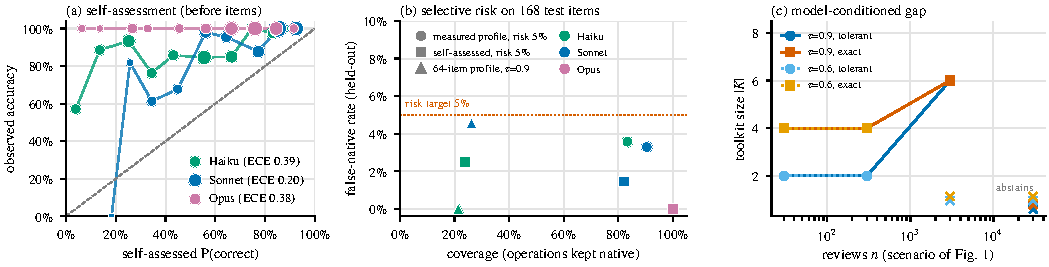
\includegraphics[width=\textwidth]{evaluation_tsc/figures/fig_rq1_profile}
\caption{Model profile: (a) self-assessment reliability, (b) coverage versus false-native rate, (c) toolkit size
versus input size (crosses: abstentions).}
\label{fig:ev-profile}
\end{figure*}

Capability boundaries differ by model and by operation (Table~\ref{tab:ev-calibration}). Haiku fails counting
from $n=40$, Sonnet loses joins as they grow, and both fail approximate sums over 640 values, whereas Opus answers
all 387 items it was given. With the measured profile and a 5\% risk target, the held-out false-native rate stays
within the target for every model (3.6\%, 3.3\% and 0.0\%) while 83--100\% of the operations remain with the model
(Fig.~\ref{fig:ev-profile}b). Both baselines fail. Self-assessment is miscalibrated for every model (ECE
0.20--0.39, all underconfident; Fig.~\ref{fig:ev-profile}a), and the 64-item profile keeps only 21--26\% of the
operations native, sending most correctly performed work to tools. The gap, in turn, behaves as designed
(Fig.~\ref{fig:ev-profile}c): two tools suffice for 30 or 300 reviews and six for 3,000, and the engine abstains
rather than return an unsupported toolkit at 30,000; without gap analysis, it abstains in every setting. On the
test tasks, the profile overrules 9.4\% of the analyst's claims that an operation is native. A measured,
risk-targeted profile therefore makes model conditioning reliable, and neither self-assessment nor a small profile
can replace it.

\subsection{Evidence-Based Eligibility under Forged and Imperfect Metadata}
\label{sec:ev-rq2}

The second experiment addresses RQ2, the restriction of discovery to tools whose safety-relevant behaviour is
evidenced. It measures whether provenance-sound eligibility (P) keeps unsafe tools away from the model, and at what
cost, under a read-only policy over 273 requests with read-only gold tools. Exp@5 is the share of requests whose
top five contain a tool that is not read-only under $J_B$, and Util@5 the share whose top five contain a gold
tool; forgery and verifier errors are simulated. Verified evidence is compared with four encodings of the
policy, namely no filter, MCP's default (annotations displayed, not enforced), annotations as a closed world, and
lexical cues, each combined with \pamcp{}'s retrieval and with MCP-Zero.

\begin{table}[t]
\centering
\caption{Exposure and utility of read-only policy encodings (\%).}
\label{tab:ev-encodings}
\scriptsize
\setlength{\tabcolsep}{2.2pt}
\begin{tabular}{@{}lrrrrrrr@{}}
\toprule
 & & & \multicolumn{2}{c}{\pamcp{} retr.} & \multicolumn{2}{c}{MCP-Zero} & $\delta{=}0.2$ \\
\cmidrule(lr){4-5}\cmidrule(lr){6-7}\cmidrule(l){8-8}
Encoding & Elig. & Unsafe & Exp@5 & Util@5 & Exp@5 & Util@5 & Exp@5 \\
\midrule
no filter & 100.0 & 120 & 42.5 & 49.8 & 26.4 & 76.6 & 43.7 \\
MCP default (display only) & 100.0 & 120 & 42.5 & 49.8 & 26.4 & 76.6 & 43.7 \\
closed-world annotations & 7.7 & 1 & 31.5 & 0.4 & 0.0 & 0.4 & 58.7 \\
lexical cues & 67.8 & 21 & 9.9 & 41.0 & 12.5 & 65.6 & 8.8 \\
verified evidence (P) & 77.0 & 0 & 0.0 & 46.2 & 0.0 & 72.2 & 5.5 \\
observed + lexical fallback & 77.0 & 0 & 0.0 & 46.2 & 0.0 & 72.2 & 5.5 \\
attested only & 26.4 & 0 & 0.0 & 16.5 & 0.0 & 18.3 & 5.8 \\
\bottomrule
\end{tabular}
\end{table}

\begin{figure*}[t]
\centering
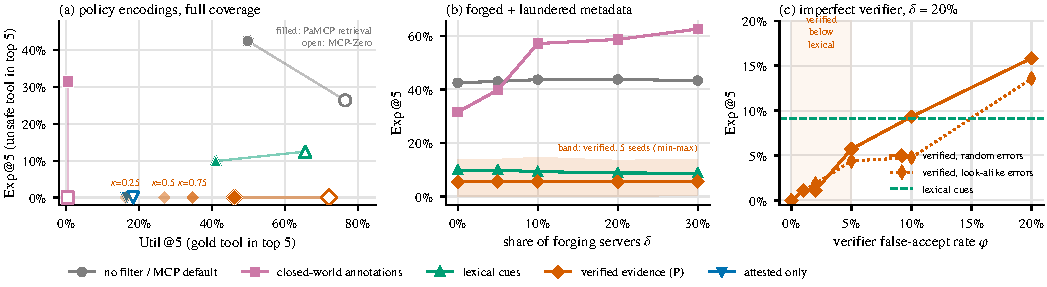
\includegraphics[width=\textwidth]{evaluation_tsc/figures/fig_rq2_exposure}
\caption{Exposure to unsafe tools: (a) policy encodings, (b) forged metadata, (c) verifier false accepts.}
\label{fig:ev-exposure}
\end{figure*}

Every baseline encoding exposes unsafe tools (Table~\ref{tab:ev-encodings}): 42.5\% of the requests without a
filter or under MCP's default, 31.5\% with annotations as a closed world (whose utility falls to 0.4\%), and 9.9\%
with lexical cues. Verified evidence admits none of the 120 unsafe tools, keeps 77\% of the registry eligible and
costs 3.6 utility points (4.4 for MCP-Zero); its difference to lexical cues is confirmatory (F4: $-9.9$ points,
$p_{\mathrm{Holm}}<0.001$). Under forgery, the closed-world reading collapses (31.5\% to 62.6\% exposure at
$\delta=0.3$), while verified evidence stays at 5.4--5.6\% for every $\delta$ with a 5\% false-accept rate
(Fig.~\ref{fig:ev-exposure}b) and remains below lexical cues up to $\varphi=5\%$ (10\% for look-alike errors;
Fig.~\ref{fig:ev-exposure}c).

\begin{figure*}[t]
\centering
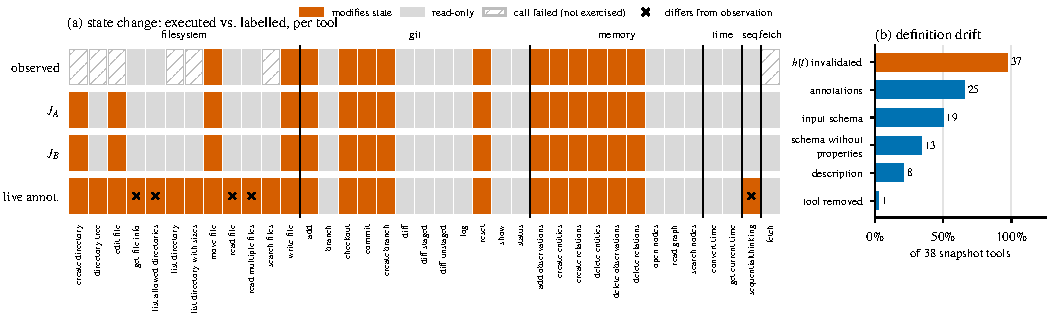
\includegraphics[width=\textwidth]{evaluation_tsc/figures/fig_rq2_observed}
\caption{Executed reference servers: (a) observed and labelled state changes, (b) definition drift since the
benchmark snapshot.}
\label{fig:ev-observed}
\end{figure*}

Three further checks remove the dependency on how the labels were built. First, with the verifier simulated from
$J_B$ and scored on $J_A$, exposure is 2.3--3.9\% across \pamcp{}, RAG-MCP, MCP-Zero and ToolScope, a quarter to
two fifths of the exposure left by lexical cues. Second, when the six MCP reference servers are executed under
system-call tracing (observed; Fig.~\ref{fig:ev-observed}), both labellings agree with all 30 completed calls: none
of the 13 tools observed to change state is labelled read-only (Wilson upper bound 22.8\%). Third, every one of the
37 surviving definitions changed since the benchmark snapshot, so evidence not bound to $h(t)$, as \pamcp{} binds
it, would have been stale. Eligibility based on verified, hash-bound evidence thus removes the exposure that
published metadata leaves, degrades in proportion to verifier error, and does not depend on the reference labels.

\subsection{Compactness and Joint Feasibility of Certified Toolkits}
\label{sec:ev-rq3}

The third experiment addresses RQ3, the return of a small toolkit whose interfaces, effects and flows are
certified jointly before any call. It examines whether set-level reasoning returns smaller toolkits that are
jointly feasible more often than retrieval on the 94 test tasks, against RAG-MCP, COLT and ToolScope (top five),
MCP-Zero, CMTF and per-subtask retrieval, each also restricted to eligible tools. Group recall is measured against
benchmark gold (measured), and joint feasibility is decided by two evaluators written independently of the
certificate: a coarse one, and a strict one that also checks domains, cardinality, schema-required inputs and
egress of private data (labelled). On ten hand-built cases with known answers, the strict evaluator decides 7
correctly and the coarse one 2.

\begin{table}[t]
\centering
\caption{Toolkit size, recall and joint feasibility on the 94 test tasks.}
\label{tab:ev-sets}
\scriptsize
\setlength{\tabcolsep}{2.1pt}
\begin{tabular}{@{}lrrlrrr@{}}
\toprule
 & & & & \multicolumn{2}{c}{Joint feas. (\%)} & \\
\cmidrule(lr){5-6}
Method & $|K|$ & Tok. & Group recall [CI] & coarse & strict & Abst. \\
\midrule
\pamcp{} ($K{=}10$) & 1.46 & 198 & 0.174 [0.12, 0.23] & 67.0 & 27.7 & 7.4 \\
\pamcp{}-L & 1.22 & 146 & 0.161 & 54.7 & 15.8 & 9.5 \\
\pamcp{} NoCert & -- & -- & -- & 59.6 & 13.8 & 0.0 \\
Per-subtask (elig.) & 2.59 & 346 & 0.249 [0.19, 0.32] & 62.8 & 8.5 & -- \\
RAG-MCP@5 (elig.) & 5.00 & 1244 & 0.293 [0.22, 0.37] & 60.6 & 5.3 & -- \\
COLT@5 (elig.) & 5.00 & 1094 & 0.295 [0.23, 0.37] & 59.6 & 8.5 & -- \\
ToolScope@5 (elig.) & 5.20 & 976 & 0.361 [0.29, 0.44] & 73.4 & 11.7 & -- \\
MCP-Zero (elig.) & 1.76 & 250 & 0.227 [0.17, 0.29] & 57.4 & 11.7 & -- \\
CMTF (elig.) & 0.64 & 105 & 0.072 [0.04, 0.11] & 25.5 & 14.9 & -- \\
RAG-MCP@5 (published) & 5.00 & 1244 & 0.293 [0.22, 0.37] & 48.9 & 5.3 & -- \\
\bottomrule
\end{tabular}
\end{table}

\begin{figure*}[t]
\centering
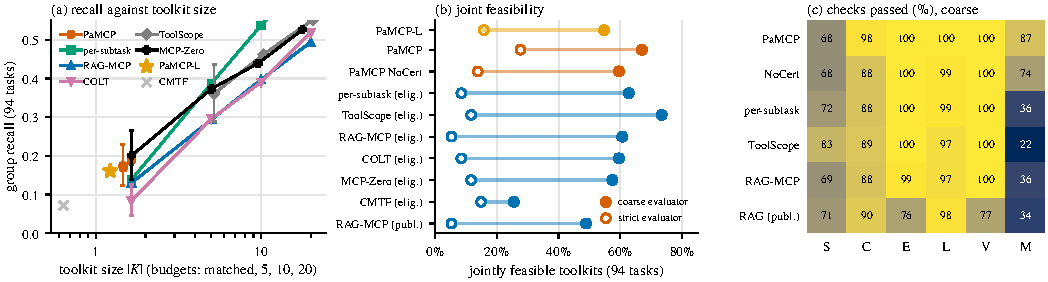
\includegraphics[width=\textwidth]{evaluation_tsc/figures/fig_rq3_sets}
\caption{Toolkit quality: (a) recall versus toolkit size, (b) joint feasibility, (c) certificate checks passed
(S goals, C inputs, E effects, L flows, V evidence, M minimality).}
\label{fig:ev-sets}
\end{figure*}

\pamcp{} returns the smallest toolkits apart from CMTF, with 1.46 tools and 198 tokens against 5 tools and
976--1,244 tokens for the top-five retrievers (Table~\ref{tab:ev-sets}), and it certifies 92.6\% of the tasks,
abstaining with a counterexample on the rest. Under the strict evaluator, its toolkits are jointly feasible in
27.7\% of the tasks, 1.9 to 5.2 times as often as every baseline restricted to eligible tools (5.3--14.9\%) and
twice as often as without certification (13.8\%; Fig.~\ref{fig:ev-sets}b). Certification acts through obtainable
inputs and minimality (C 88\% to 98\%, M 74\% to 87\%, against 22--36\% for the top-five retrievers;
Fig.~\ref{fig:ev-sets}c). At equal size, \pamcp{} reaches more gold steps than RAG-MCP, per-subtask retrieval and
COLT (0.189 against 0.130, 0.138 and 0.084; F2 not significant after correction), whereas retrievers that expose
three to four times more tools reach more (0.249--0.361; non-inferiority to per-subtask retrieval, F1, not shown).
\pamcp{} thus trades breadth for certified compactness.

\begin{table}[t]
\centering
\caption{Single-tool retrieval accuracy on the 300 test requests.}
\label{tab:ev-retrieval}
\scriptsize
\setlength{\tabcolsep}{2.4pt}
\begin{tabular}{@{}lrrrrrr@{}}
\toprule
 & 81 tools & \multicolumn{5}{c}{569 tools} \\
\cmidrule(lr){2-2}\cmidrule(l){3-7}
Method & Hit@1 & Hit@1 [CI] & Hit@3 & Hit@5 & MRR & nDCG \\
\midrule
BM25 & 52.7 & 41.0 [26, 60] & 57.3 & 63.7 & 0.503 & 0.543 \\
RAG-MCP (dense) & 49.7 & 37.3 [22, 56] & 50.0 & 54.3 & 0.451 & 0.492 \\
RRF fusion & 54.3 & 38.7 [23, 57] & 54.7 & 61.3 & 0.481 & 0.525 \\
MCP-Zero & 68.0 & 66.7 [49, 80] & 80.0 & 85.7 & 0.743 & 0.775 \\
COLT & 49.7 & 37.3 [22, 56] & 50.0 & 54.3 & 0.451 & 0.492 \\
ToolScope & 53.0 & 41.0 [26, 60] & 58.3 & 63.7 & 0.504 & 0.543 \\
CMTF & 58.7 & 32.7 [19, 49] & 47.0 & 54.7 & 0.428 & 0.488 \\
PaMCP (Eq. 5) & 61.0 & 29.7 [16, 47] & 45.7 & 53.7 & 0.400 & 0.461 \\
PaMCP-L & 72.0 & 41.3 [25, 60] & 61.3 & 69.3 & 0.536 & 0.603 \\
PaMCP, oracle types (diag.) & 71.7 & 58.3 [38, 74] & 75.3 & 81.3 & 0.680 & 0.728 \\
\bottomrule
\end{tabular}
\end{table}

Single-tool retrieval, in contrast, is not where \pamcp{} gains (Table~\ref{tab:ev-retrieval}). Over 81 tools, its
relevance-first ranking is the most accurate (72.0\% Hit@1, against 68.0\% for MCP-Zero), but over the full
registry MCP-Zero leads (66.7\%), \pamcp{}-L ties tuned BM25 (41.3\% against 41.0\%; H1 n.s.), and the structural
ranking of Eq.~(5) falls to 29.7\% (F7 against \pamcp{}), because types agree with $J_B$ on 78.9\% of output kinds
but only on 35.7\% of domains. With correct types, the same ranking reaches 58.3\%, above every baseline except
MCP-Zero, which locates the limit in the typing rather than in the composition. Set-level reasoning therefore
yields the most compact and most often jointly feasible toolkits, while finding more tools requires better typing
or a larger budget.

\subsection{Resistance to Injected Actions and Contribution of the Mechanisms}
\label{sec:ev-sec}

The fourth experiment combines RQ2 and RQ3. It measures whether the exposed
toolkit limits what an injected instruction could achieve, and which mechanism is responsible. For 155 tasks and
each attack class outside the task's needs, an attack is reachable if the toolkit can realise it under $J_B$
(labelled, offline). Poisoning places a canary in the description, name or argument keys of 10--30\% of the tools,
and we scan what each method shows the model; the mechanisms are varied in a $2^3$ design with Shapley
attribution.

\begin{figure*}[t]
\centering
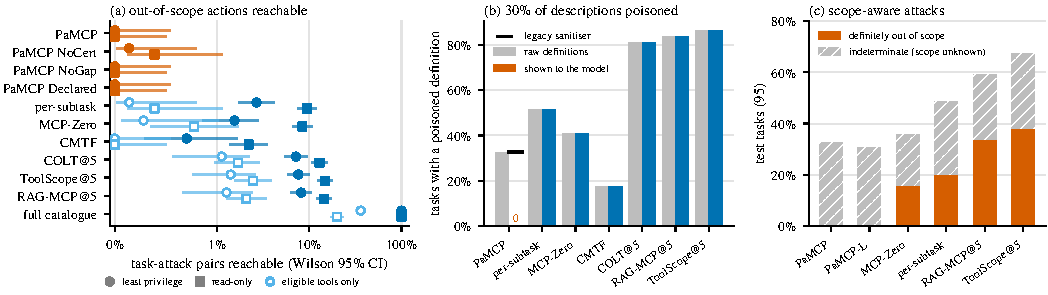
\includegraphics[width=\textwidth]{evaluation_tsc/figures/fig_sec_injection}
\caption{Injected actions: (a) reachable out-of-scope actions, (b) poisoned definitions shown to the model,
(c) scope of admitted attacks.}
\label{fig:ev-injection}
\end{figure*}

No out-of-scope action is reachable through \pamcp{}'s toolkits: 0 of 712 task--attack pairs under least privilege
and 0 of 775 under a read-only policy, against 0.7--8.1\% and 8.4--14.7\% for the published baselines
(Fig.~\ref{fig:ev-injection}a; F5, $p_{\mathrm{Holm}}<0.001$). Counting only attacks that are definitely out of
scope, no \pamcp{} toolkit admits one, against 15.8\% of the tasks for MCP-Zero, 20.0\% for per-subtask retrieval,
33.7\% for RAG-MCP and 37.9\% for ToolScope (H5: $-20.0$ points, 95\% CI $[-28.4,-12.6]$,
$p_{\mathrm{Holm}}<0.001$), although 32.6\% admit an attack whose scope the labels cannot decide. With 30\% of the
descriptions poisoned, the aliased manifest never shows an injected instruction, whereas the definitions exposed
by the baselines carry one in 17.4--86.2\% of the tasks (Fig.~\ref{fig:ev-injection}b). Moreover, 55.5\% of
\pamcp{}'s toolkits return remote content, but none of them also enables an out-of-scope action, against
3.2--22.6\% for the baselines.

\begin{table}[t]
\centering
\caption{Ablation of the gap (G), eligibility (P) and set reasoning (S).}
\label{tab:ev-factorial}
\scriptsize
\setlength{\tabcolsep}{3pt}
\begin{tabular}{@{}cccrrrrr@{}}
\toprule
G & P & S & Recall & Tokens & Joint (\%) & Reach (\%) & Abst. (\%) \\
\midrule
-- & -- & -- & 0.270 & 297 & 53.5 & 1.1 & 0.0 \\
on & -- & -- & 0.239 & 208 & 55.5 & 0.4 & 0.0 \\
-- & on & -- & 0.295 & 316 & 58.1 & 0.1 & 0.0 \\
-- & -- & on & 0.223 & 221 & 52.9 & 0.1 & 16.1 \\
on & on & -- & 0.253 & 229 & 56.8 & 0.1 & 0.0 \\
on & -- & on & 0.230 & 189 & 54.8 & 0.0 & 6.5 \\
-- & on & on & 0.183 & 193 & 55.5 & 0.0 & 20.0 \\
on & on & on & 0.181 & 176 & 56.1 & 0.0 & 10.3 \\
\midrule
\multicolumn{3}{@{}l}{Full, no backward closure} & 0.181 & 173 & 53.5 & 0.0 & 12.3 \\
\multicolumn{3}{@{}l}{Full, flow along derivations} & 0.236 & 206 & 60.6 & 0.0 & 5.8 \\
\multicolumn{3}{@{}l}{Full, no relevance term} & 0.167 & 141 & 54.8 & 0.0 & 10.3 \\
\multicolumn{3}{@{}l}{Full, no utility floor} & 0.181 & 176 & 56.1 & 0.0 & 10.3 \\
\multicolumn{3}{@{}l}{Full, no refinement} & 0.179 & 175 & 55.5 & 0.0 & 11.0 \\
\bottomrule
\end{tabular}
\end{table}

The factorial design (Table~\ref{tab:ev-factorial}) shows that each mechanism contributes. Eligibility removes
most reachable actions, and with gap analysis and set reasoning, reachability falls from 5.2\% of the tasks to none
(Shapley shares of 23\%, 35\% and 42\% for G, P and S). Gap analysis and set reasoning shrink the context from 297
to 176 tokens (main effects of $-56$ and $-67$ tokens, $p<0.001$), and the gap halves abstentions (10.3\% against
20.0\%). The price is recall (0.270 to 0.181, mainly through S), and no mechanism changes the coarse joint
feasibility. Under the labelled threat model, \pamcp{}'s mechanisms therefore jointly close the action and
metadata channels that retrieval baselines leave open.

\subsection{Scalability, Optimality and Adaptation to Registry Change}
\label{sec:ev-eff}

The last experiment addresses RQ4, discovery at a cost that scales and under registry change, together with the
optimality of the composition studied under RQ3. It measures what discovery costs, how close the composition is
to the optimum, and whether the engine keeps its guarantees under change. The engine is compared with eager
materialisation of the risk relation, with the greedy regime and an integer program (HiGHS) written independently
of the engine, with full rebuilds and cache flushes, and with cold discovery without experience reuse.

\begin{figure*}[t]
\centering
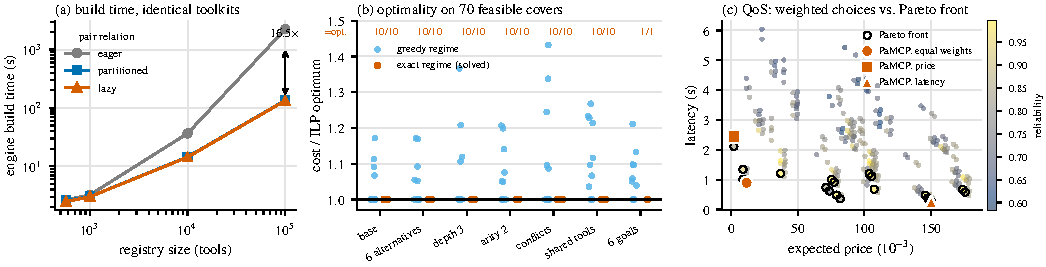
\includegraphics[width=\textwidth]{evaluation_tsc/figures/fig_tsc_eff}
\caption{Efficiency: (a) engine build time by pair-relation mode, (b) cost relative to the ILP optimum, (c) QoS
choices and Pareto front.}
\label{fig:ev-eff}
\end{figure*}

On the real registry, a request takes 49\,ms at the median (eligibility 0.08\,ms, against 12\,ms for RAG-MCP's
single dense ranking) and 2.7\,s at $10^5$ cloned tools. Deciding the pairwise risk relation lazily or by effect
class gives identical toolkits on all test tasks and builds the engine at $10^5$ tools in 133--134\,s instead of
2,224\,s, 16.5 times faster with near-linear growth (Fig.~\ref{fig:ev-eff}a); on heterogeneous registries of
$10^4$ tools, the lazy build takes 4.6--5.9\,s. Wherever the exact search finishes, it returns the ILP optimum (61
of 61 solved instances across alternatives, depth, arity, conflicts and shared tools) and recognises all ten
infeasible instances, while the greedy regime is 4.4--12.6\% above the optimum on average
(Fig.~\ref{fig:ev-eff}b); with six goals, the search exhausts its budget and falls back to greedy (6.9\% above).
When providers differ in price, latency and reliability, every equal-weight choice is Pareto-optimal and meets the
utility floor, and the weights move the choice along the front as intended (price only: 0.33$\times$ price;
latency only: 0.73$\times$ latency; Fig.~\ref{fig:ev-eff}c).

The engine also adapts to change at low cost. An incremental update takes 13.5\,ms against 4.2\,s for a rebuild,
the exact invalidation of Proposition~3 touches 1.1\% of the cached toolkits instead of all of them, and all 20
simulated rug pulls lose their evidence. Experience reuse serves 32.7\% of 300 requests without an analyst call,
with unchanged certification (82.7\% against 82.3\%) and no violation in 89 revalidation probes (removed servers,
revoked or rewritten tools, stricter principal, other model). Deterministic repair raises certification from
72.6\% to 87.4\% when counterexamples are induced. The complete engine thus scales to $10^5$ tools, composes
optimally where it searches exactly, makes Pareto-consistent QoS trade-offs and adapts to change without losing
its guarantees.

\subsection{Summary of Findings and Threats to Validity}
\label{sec:ev-threats}

\begin{table}[t]
\centering
\caption{Summary of findings (Conf.: confirmatory test, $p_{\mathrm{Holm}}$).}
\label{tab:ev-answers}
\scriptsize
\setlength{\tabcolsep}{2pt}
\begin{tabular}{@{}lp{2.85cm}p{2.95cm}l@{}}
\toprule
Aspect & Result & Best baseline & Conf. \\
\midrule
Profile & FNR $\le$3.6\% at 83--100\% coverage & self-assessment ECE 0.20--0.39 & -- \\
Eligibility & Exp@5 0\% (swap 2.3--3.9\%), Util $-3.6$ & lexical 9.9\%, MCP default 42.5\% & F4 $<$0.001 \\
Execution & labels = execution, 30/30 calls & -- (observed) & -- \\
Feasibility & strict joint 27.7\%, 1.46 tools & 5.3--14.9\%, 0.64--5.2 tools & expl. \\
Recall & recall at equal size 0.189 & 0.084--0.200 & F2 n.s. \\
Retrieval & Hit@1 (569) 41.3\% & MCP-Zero 66.7\% & F7 against \\
Security & reachable 0/712, definite 0\% & 0.7--8.1\%, 15.8--37.9\% & F5, H5 $<$0.001 \\
Scaling & build 16.5$\times$ faster; =ILP 61/61 & eager 2,224\,s; greedy +4--13\% & -- \\
Evolution & update 13.5\,ms; reuse 32.7\% & rebuild 4.2\,s; cold & -- \\
\bottomrule
\end{tabular}
\end{table}

\begin{table}[t]
\centering
\caption{Confirmatory comparisons (Holm-corrected; $\Delta$: \pamcp{} minus comparator, in points, tokens for F6).}
\label{tab:ev-family}
\scriptsize
\setlength{\tabcolsep}{2.2pt}
\begin{tabular}{@{}llrlll@{}}
\toprule
 & Comparison & $\Delta$ & 95\% CI & $p_{\mathrm{Holm}}$ & Verdict \\
\midrule
F1 & Group recall vs per-subtask (non-inf., 0.05) & -8.0 & [-16.6, +0.2] & 1.000 & not shown \\
F2 & Size-matched recall vs RAG-MCP & +6.0 & [-1.6, +13.7] & 0.397 & n.s. \\
F3 & Joint feasibility vs per-subtask (elig.) & +4.3 & [-8.5, +18.1] & 1.000 & n.s. \\
F4 & Exp@5 verified vs lexical & -9.9 & [-13.9, -6.6] & $<$0.001 & supports \\
F5 & Reachable attacks vs per-subtask & -2.7 & [-3.9, -1.5] & $<$0.001 & supports \\
F6 & Tokens, full vs NoGap & -16.7 & [-34.6, +1.0] & 0.269 & n.s. \\
F7 & Hit@1 goal contract vs raw RRF (569) & -15.7 & [-21.3, -10.0] & $<$0.001 & against \\
\midrule
H1 & Hit@1 PaMCP-L vs tuned BM25 (569) & +0.3 & [-8.9, +8.8] & 1.000 & n.s. \\
H2 & Hit@1 PaMCP-L vs Eq. (5) (569) & +11.7 & [+3.0, +22.6] & 0.070 & n.s. \\
H3 & Group recall PaMCP-L vs per-subtask (non-inf.) & -8.8 & [-17.6, -0.5] & 1.000 & not shown \\
H4 & Strict joint feas. vs per-subtask (elig.) & +7.4 & [+0.0, +14.9] & 0.277 & n.s. \\
H5 & Definite out-of-scope vs per-subtask & -20.0 & [-28.4, -12.6] & $<$0.001 & supports \\
\bottomrule
\end{tabular}
\end{table}

Table~\ref{tab:ev-answers} summarises the findings for RQ1--RQ4, and Table~\ref{tab:ev-family} the confirmatory
tests. All confirmatory tests on safety (F4, F5 and H5) favour \pamcp{} at $p_{\mathrm{Holm}}<0.001$; the tests on
recall and retrieval do not, and the feasibility advantage under the strict evaluator is exploratory.

These findings are subject to several threats to validity. Effects, types and feasibility are scored against LLM
labels; execution confirms them on 30 calls of six non-adversarial reference servers, and the label swap bounds
the effect of labeller disagreement but not of errors shared by one model family. Reachability is decided offline:
whether an agent follows an injected instruction, and end-to-end task success, require executing the toolkits,
which this study did not do. The baselines are adaptations sharing a TF-IDF and SVD encoder, all tuned on the same
development split; larger registries are cloned or generated, and QoS data are synthetic. Executed compositions
over isolated and adversarial servers, human annotation of a stratified tool sample and reproductions of the
baselines with their original encoders are the natural next steps, and the released artifact supports each of
them.
; needs graphicx, booktabs, amsmath, url.
% Generated by paper/package_overleaf.py from paper/sections/evaluation_tsc.tex
% (repository msellamiTN/taas-provenance-discovery, branch research/pamcp-final-evaluation).
\providecommand{\pamcp}{PaMCP}
\section{Experimental Evaluation}
\label{sec:ev}

This section evaluates \pamcp{} against the strongest baselines we could configure. Every result is labelled by
its evidence class: \emph{measured} from the running system, \emph{observed} from executed servers,
\emph{labelled} against reference labels, or \emph{simulated} under stated assumptions; the main comparisons are
confirmed with pre-registered tests.

\subsection{Datasets, Baselines and Evaluation Protocol}
\label{sec:ev-setup}

\begin{table}[t]
\centering
\caption{Datasets and compared methods.}
\label{tab:ev-setup}
\scriptsize
\setlength{\tabcolsep}{2.5pt}
\begin{tabular}{@{}p{2.3cm}p{5.65cm}@{}}
\toprule
\multicolumn{2}{@{}l}{\emph{Data}} \\
Registry & 569 tools, 76 servers (LiveMCPTool \cite{mo2025livemcpbench} + MCPToolBench++ \cite{fan2025mcptoolbench}); 44 annotated \\
Multi-step tasks & 95 LiveMCPBench tasks (test); 60 development prompts \\
Single-tool requests & 60 development / 300 test (50 per category, 66 targets) \\
Calibration suite & 432 items: 6 operations, $n\in\{10,40,160,640\}$, en/fr, noise, context; 264 cal.\ / 168 test \\
Executed servers & 6 MCP reference servers, 37 registry tools \\
Synthetic & cloned and heterogeneous registries ($10^3$--$10^5$); 80 cover and 120 QoS instances \\
\midrule
\multicolumn{2}{@{}l}{\emph{Baselines (adapted to one registry, one encoder; tuned on the development split)}} \\
RAG-MCP \cite{gan2025ragmcp} & dense top-$k$ over the request \\
MCP-Zero \cite{fei2025mcpzero} & model-written requests, server routing \\
COLT \cite{qu2024colt} & collaborative graph of 450 training queries \\
ToolScope \cite{liu2026toolscope} & LLM-confirmed tool merging, subquery retrieval \\
CMTF \cite{suresh2026cmtf} & typed-state search, one tool per step \\
BM25, RRF, per-subtask & lexical, fused, one tool per analyst subgoal \\
\midrule
\multicolumn{2}{@{}l}{\emph{Ablations of \pamcp{}}} \\
G, P, S & gap (Alg.~1), eligibility (Sec.~5), set reasoning + certificate (Sec.~6), $2^3$ design \\
\pamcp{}-L & relevance-first ranking selected on the development split \\
\bottomrule
\end{tabular}
\end{table}

\begin{table}[t]
\centering
\caption{Experimental parameters (defaults in bold).}
\label{tab:ev-params}
\scriptsize
\setlength{\tabcolsep}{2.5pt}
\begin{tabular}{@{}lp{4.3cm}@{}}
\toprule
Parameter & Values \\
\midrule
Profile threshold $\tau$ / risk target & 0.6, 0.75, \textbf{0.9} / 0.05, 0.10 \\
Forging servers $\delta$; false accepts $\varphi$ & 0--0.3 (5 seeds); 0--0.2, \textbf{0.05} \\
Probe coverage $\kappa$; trust $\ell_{\min}$ & 0.25--\textbf{1}; 0.2--0.95, \textbf{0.65} \\
Candidate budget $K$; size matching & 1, 5, \textbf{10}, 20, 40; equal $|K|$ \\
Poisoned descriptions; policies & 10\%, 30\%; least privilege, read-only \\
Registry size; pair relation & 569--$10^5$; eager, partitioned, \textbf{lazy} \\
Cost weights; utility floor $u_{\min}$ & 0, 0.25, \textbf{0.5}, 1; 0--0.9 \\
\bottomrule
\end{tabular}
\end{table}

Table~\ref{tab:ev-setup} lists the data and the compared methods, and Table~\ref{tab:ev-params} the parameters
varied across the experiments. Effects and types are scored against blind labels $J_B$ (Claude Opus), which are
not used to simulate evidence; the simulated verifier uses labels $J_A$ (Claude Sonnet), and we report the
swapped direction and executed servers to remove the dependency between the two. All LLM outputs were recorded
once and are replayed, and every method, including \pamcp{}, was configured on the development split only.
Request-level metrics are resampled with target tools as clusters and task-level metrics with tasks; paired tests
are sign-flip permutation tests, and proportions use Wilson intervals (95\%). Two confirmatory families (F1--F7,
H1--H5) were fixed before the data they test and are Holm-corrected. Code, records, manifests and a notebook that
re-runs every experiment on a CPU are public.\footnote{\url{https://github.com/msellamiTN/taas-provenance-discovery},
branch \texttt{research/pamcp-final-evaluation}; guide in \texttt{docs/REPRODUCIBILITY.md}.}

\subsection{Measured Model Profiles for Model-Conditioned Discovery}
\label{sec:ev-rq1}

The first experiment addresses RQ1, the conditioning of discovery on the deployed model. It tests whether a
measured profile $\rho_{\mathrm{LLM}}$ decides reliably which operations the deployed model keeps, and whether the
gap responds to the model and to the input. Three models answer the calibration suite by reading only, after
stating for each cell their probability of success; $\tau$ is chosen on the calibration split for a risk target
and evaluated on held-out items (measured). The measured profile is compared with two baselines, the model's own
self-assessment and the earlier 64-item profile.

\begin{table}[t]
\centering
\caption{Calibration of the model profile (Cov.: operations kept native; FNR: false-native rate).}
\label{tab:ev-calibration}
\scriptsize
\setlength{\tabcolsep}{2.2pt}
\begin{tabular}{@{}lrcrrrrrrrr@{}}
\toprule
 & & & & \multicolumn{2}{c}{Self-assess.} & \multicolumn{3}{c}{Measured, risk 5\%} & \multicolumn{2}{c}{64-item} \\
\cmidrule(lr){5-6}\cmidrule(lr){7-9}\cmidrule(l){10-11}
Model & $n$ & Accuracy (\%) & $n{=}640$ & ECE & Brier & $\tau$ & Cov. & FNR & Cov. & FNR \\
\midrule
Haiku & 432 & 86.1 [82.5, 89.1] & 67 & 0.39 & 0.30 & 0.21 & 83 & 3.6 & 21 & 0.0 \\
Sonnet & 432 & 91.4 [88.4, 93.7] & 62 & 0.20 & 0.11 & 0.42 & 90 & 3.3 & 26 & 4.5 \\
Opus & 387 & 100.0 [99.0, 100.0] & 100 & 0.38 & 0.20 & 0.90 & 100 & 0.0 & -- & -- \\
\bottomrule
\end{tabular}
\end{table}

\begin{figure*}[t]
\centering
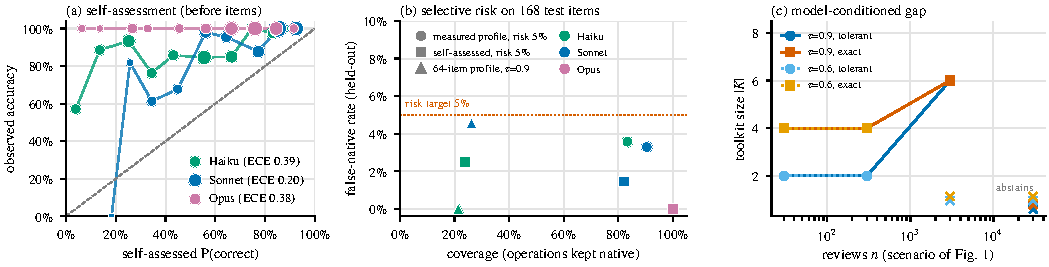
\includegraphics[width=\textwidth]{evaluation_tsc/figures/fig_rq1_profile}
\caption{Model profile: (a) self-assessment reliability, (b) coverage versus false-native rate, (c) toolkit size
versus input size (crosses: abstentions).}
\label{fig:ev-profile}
\end{figure*}

Capability boundaries differ by model and by operation (Table~\ref{tab:ev-calibration}). Haiku fails counting
from $n=40$, Sonnet loses joins as they grow, and both fail approximate sums over 640 values, whereas Opus answers
all 387 items it was given. With the measured profile and a 5\% risk target, the held-out false-native rate stays
within the target for every model (3.6\%, 3.3\% and 0.0\%) while 83--100\% of the operations remain with the model
(Fig.~\ref{fig:ev-profile}b). Both baselines fail. Self-assessment is miscalibrated for every model (ECE
0.20--0.39, all underconfident; Fig.~\ref{fig:ev-profile}a), and the 64-item profile keeps only 21--26\% of the
operations native, sending most correctly performed work to tools. The gap, in turn, behaves as designed
(Fig.~\ref{fig:ev-profile}c): two tools suffice for 30 or 300 reviews and six for 3,000, and the engine abstains
rather than return an unsupported toolkit at 30,000; without gap analysis, it abstains in every setting. On the
test tasks, the profile overrules 9.4\% of the analyst's claims that an operation is native. A measured,
risk-targeted profile therefore makes model conditioning reliable, and neither self-assessment nor a small profile
can replace it.

\subsection{Evidence-Based Eligibility under Forged and Imperfect Metadata}
\label{sec:ev-rq2}

The second experiment addresses RQ2, the restriction of discovery to tools whose safety-relevant behaviour is
evidenced. It measures whether provenance-sound eligibility (P) keeps unsafe tools away from the model, and at what
cost, under a read-only policy over 273 requests with read-only gold tools. Exp@5 is the share of requests whose
top five contain a tool that is not read-only under $J_B$, and Util@5 the share whose top five contain a gold
tool; forgery and verifier errors are simulated. Verified evidence is compared with four encodings of the
policy, namely no filter, MCP's default (annotations displayed, not enforced), annotations as a closed world, and
lexical cues, each combined with \pamcp{}'s retrieval and with MCP-Zero.

\begin{table}[t]
\centering
\caption{Exposure and utility of read-only policy encodings (\%).}
\label{tab:ev-encodings}
\scriptsize
\setlength{\tabcolsep}{2.2pt}
\begin{tabular}{@{}lrrrrrrr@{}}
\toprule
 & & & \multicolumn{2}{c}{\pamcp{} retr.} & \multicolumn{2}{c}{MCP-Zero} & $\delta{=}0.2$ \\
\cmidrule(lr){4-5}\cmidrule(lr){6-7}\cmidrule(l){8-8}
Encoding & Elig. & Unsafe & Exp@5 & Util@5 & Exp@5 & Util@5 & Exp@5 \\
\midrule
no filter & 100.0 & 120 & 42.5 & 49.8 & 26.4 & 76.6 & 43.7 \\
MCP default (display only) & 100.0 & 120 & 42.5 & 49.8 & 26.4 & 76.6 & 43.7 \\
closed-world annotations & 7.7 & 1 & 31.5 & 0.4 & 0.0 & 0.4 & 58.7 \\
lexical cues & 67.8 & 21 & 9.9 & 41.0 & 12.5 & 65.6 & 8.8 \\
verified evidence (P) & 77.0 & 0 & 0.0 & 46.2 & 0.0 & 72.2 & 5.5 \\
observed + lexical fallback & 77.0 & 0 & 0.0 & 46.2 & 0.0 & 72.2 & 5.5 \\
attested only & 26.4 & 0 & 0.0 & 16.5 & 0.0 & 18.3 & 5.8 \\
\bottomrule
\end{tabular}
\end{table}

\begin{figure*}[t]
\centering
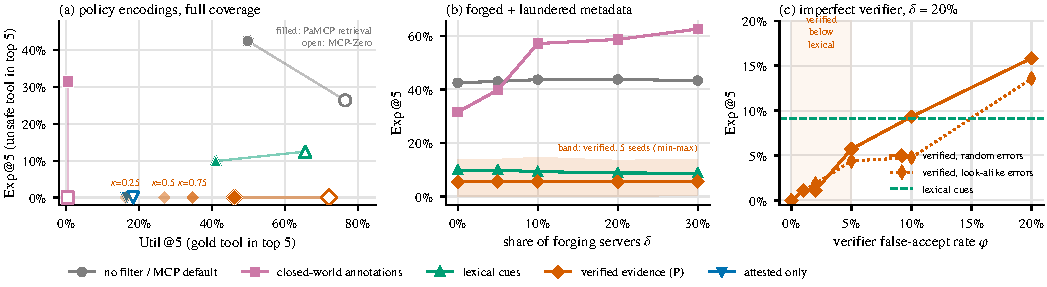
\includegraphics[width=\textwidth]{evaluation_tsc/figures/fig_rq2_exposure}
\caption{Exposure to unsafe tools: (a) policy encodings, (b) forged metadata, (c) verifier false accepts.}
\label{fig:ev-exposure}
\end{figure*}

Every baseline encoding exposes unsafe tools (Table~\ref{tab:ev-encodings}): 42.5\% of the requests without a
filter or under MCP's default, 31.5\% with annotations as a closed world (whose utility falls to 0.4\%), and 9.9\%
with lexical cues. Verified evidence admits none of the 120 unsafe tools, keeps 77\% of the registry eligible and
costs 3.6 utility points (4.4 for MCP-Zero); its difference to lexical cues is confirmatory (F4: $-9.9$ points,
$p_{\mathrm{Holm}}<0.001$). Under forgery, the closed-world reading collapses (31.5\% to 62.6\% exposure at
$\delta=0.3$), while verified evidence stays at 5.4--5.6\% for every $\delta$ with a 5\% false-accept rate
(Fig.~\ref{fig:ev-exposure}b) and remains below lexical cues up to $\varphi=5\%$ (10\% for look-alike errors;
Fig.~\ref{fig:ev-exposure}c).

\begin{figure*}[t]
\centering
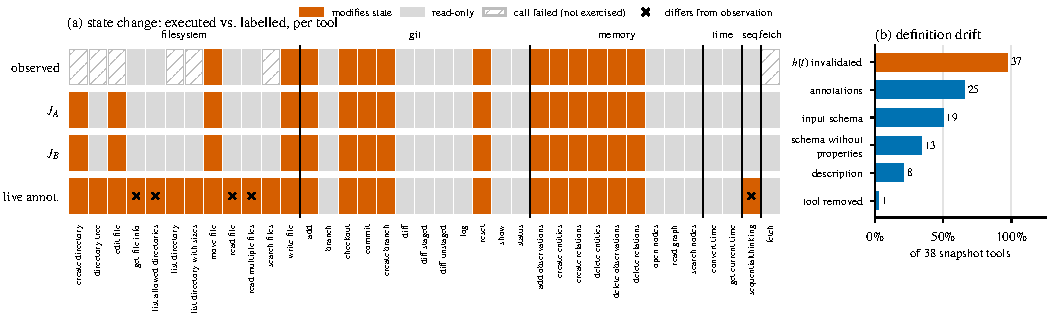
\includegraphics[width=\textwidth]{evaluation_tsc/figures/fig_rq2_observed}
\caption{Executed reference servers: (a) observed and labelled state changes, (b) definition drift since the
benchmark snapshot.}
\label{fig:ev-observed}
\end{figure*}

Three further checks remove the dependency on how the labels were built. First, with the verifier simulated from
$J_B$ and scored on $J_A$, exposure is 2.3--3.9\% across \pamcp{}, RAG-MCP, MCP-Zero and ToolScope, a quarter to
two fifths of the exposure left by lexical cues. Second, when the six MCP reference servers are executed under
system-call tracing (observed; Fig.~\ref{fig:ev-observed}), both labellings agree with all 30 completed calls: none
of the 13 tools observed to change state is labelled read-only (Wilson upper bound 22.8\%). Third, every one of the
37 surviving definitions changed since the benchmark snapshot, so evidence not bound to $h(t)$, as \pamcp{} binds
it, would have been stale. Eligibility based on verified, hash-bound evidence thus removes the exposure that
published metadata leaves, degrades in proportion to verifier error, and does not depend on the reference labels.

\subsection{Compactness and Joint Feasibility of Certified Toolkits}
\label{sec:ev-rq3}

The third experiment addresses RQ3, the return of a small toolkit whose interfaces, effects and flows are
certified jointly before any call. It examines whether set-level reasoning returns smaller toolkits that are
jointly feasible more often than retrieval on the 94 test tasks, against RAG-MCP, COLT and ToolScope (top five),
MCP-Zero, CMTF and per-subtask retrieval, each also restricted to eligible tools. Group recall is measured against
benchmark gold (measured), and joint feasibility is decided by two evaluators written independently of the
certificate: a coarse one, and a strict one that also checks domains, cardinality, schema-required inputs and
egress of private data (labelled). On ten hand-built cases with known answers, the strict evaluator decides 7
correctly and the coarse one 2.

\begin{table}[t]
\centering
\caption{Toolkit size, recall and joint feasibility on the 94 test tasks.}
\label{tab:ev-sets}
\scriptsize
\setlength{\tabcolsep}{2.1pt}
\begin{tabular}{@{}lrrlrrr@{}}
\toprule
 & & & & \multicolumn{2}{c}{Joint feas. (\%)} & \\
\cmidrule(lr){5-6}
Method & $|K|$ & Tok. & Group recall [CI] & coarse & strict & Abst. \\
\midrule
\pamcp{} ($K{=}10$) & 1.46 & 198 & 0.174 [0.12, 0.23] & 67.0 & 27.7 & 7.4 \\
\pamcp{}-L & 1.22 & 146 & 0.161 & 54.7 & 15.8 & 9.5 \\
\pamcp{} NoCert & -- & -- & -- & 59.6 & 13.8 & 0.0 \\
Per-subtask (elig.) & 2.59 & 346 & 0.249 [0.19, 0.32] & 62.8 & 8.5 & -- \\
RAG-MCP@5 (elig.) & 5.00 & 1244 & 0.293 [0.22, 0.37] & 60.6 & 5.3 & -- \\
COLT@5 (elig.) & 5.00 & 1094 & 0.295 [0.23, 0.37] & 59.6 & 8.5 & -- \\
ToolScope@5 (elig.) & 5.20 & 976 & 0.361 [0.29, 0.44] & 73.4 & 11.7 & -- \\
MCP-Zero (elig.) & 1.76 & 250 & 0.227 [0.17, 0.29] & 57.4 & 11.7 & -- \\
CMTF (elig.) & 0.64 & 105 & 0.072 [0.04, 0.11] & 25.5 & 14.9 & -- \\
RAG-MCP@5 (published) & 5.00 & 1244 & 0.293 [0.22, 0.37] & 48.9 & 5.3 & -- \\
\bottomrule
\end{tabular}
\end{table}

\begin{figure*}[t]
\centering
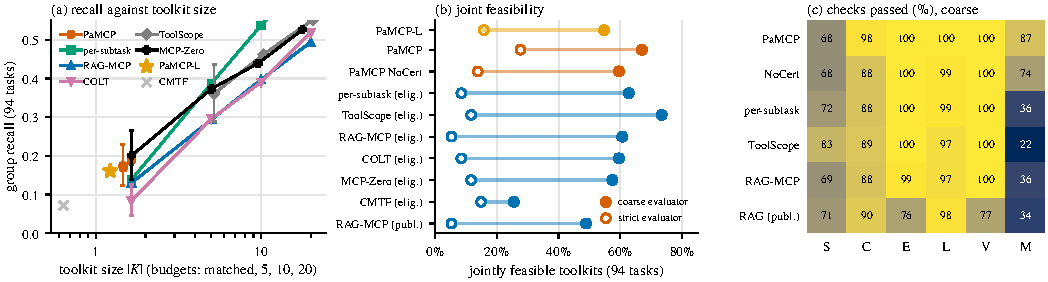
\includegraphics[width=\textwidth]{evaluation_tsc/figures/fig_rq3_sets}
\caption{Toolkit quality: (a) recall versus toolkit size, (b) joint feasibility, (c) certificate checks passed
(S goals, C inputs, E effects, L flows, V evidence, M minimality).}
\label{fig:ev-sets}
\end{figure*}

\pamcp{} returns the smallest toolkits apart from CMTF, with 1.46 tools and 198 tokens against 5 tools and
976--1,244 tokens for the top-five retrievers (Table~\ref{tab:ev-sets}), and it certifies 92.6\% of the tasks,
abstaining with a counterexample on the rest. Under the strict evaluator, its toolkits are jointly feasible in
27.7\% of the tasks, 1.9 to 5.2 times as often as every baseline restricted to eligible tools (5.3--14.9\%) and
twice as often as without certification (13.8\%; Fig.~\ref{fig:ev-sets}b). Certification acts through obtainable
inputs and minimality (C 88\% to 98\%, M 74\% to 87\%, against 22--36\% for the top-five retrievers;
Fig.~\ref{fig:ev-sets}c). At equal size, \pamcp{} reaches more gold steps than RAG-MCP, per-subtask retrieval and
COLT (0.189 against 0.130, 0.138 and 0.084; F2 not significant after correction), whereas retrievers that expose
three to four times more tools reach more (0.249--0.361; non-inferiority to per-subtask retrieval, F1, not shown).
\pamcp{} thus trades breadth for certified compactness.

\begin{table}[t]
\centering
\caption{Single-tool retrieval accuracy on the 300 test requests.}
\label{tab:ev-retrieval}
\scriptsize
\setlength{\tabcolsep}{2.4pt}
\begin{tabular}{@{}lrrrrrr@{}}
\toprule
 & 81 tools & \multicolumn{5}{c}{569 tools} \\
\cmidrule(lr){2-2}\cmidrule(l){3-7}
Method & Hit@1 & Hit@1 [CI] & Hit@3 & Hit@5 & MRR & nDCG \\
\midrule
BM25 & 52.7 & 41.0 [26, 60] & 57.3 & 63.7 & 0.503 & 0.543 \\
RAG-MCP (dense) & 49.7 & 37.3 [22, 56] & 50.0 & 54.3 & 0.451 & 0.492 \\
RRF fusion & 54.3 & 38.7 [23, 57] & 54.7 & 61.3 & 0.481 & 0.525 \\
MCP-Zero & 68.0 & 66.7 [49, 80] & 80.0 & 85.7 & 0.743 & 0.775 \\
COLT & 49.7 & 37.3 [22, 56] & 50.0 & 54.3 & 0.451 & 0.492 \\
ToolScope & 53.0 & 41.0 [26, 60] & 58.3 & 63.7 & 0.504 & 0.543 \\
CMTF & 58.7 & 32.7 [19, 49] & 47.0 & 54.7 & 0.428 & 0.488 \\
PaMCP (Eq. 5) & 61.0 & 29.7 [16, 47] & 45.7 & 53.7 & 0.400 & 0.461 \\
PaMCP-L & 72.0 & 41.3 [25, 60] & 61.3 & 69.3 & 0.536 & 0.603 \\
PaMCP, oracle types (diag.) & 71.7 & 58.3 [38, 74] & 75.3 & 81.3 & 0.680 & 0.728 \\
\bottomrule
\end{tabular}
\end{table}

Single-tool retrieval, in contrast, is not where \pamcp{} gains (Table~\ref{tab:ev-retrieval}). Over 81 tools, its
relevance-first ranking is the most accurate (72.0\% Hit@1, against 68.0\% for MCP-Zero), but over the full
registry MCP-Zero leads (66.7\%), \pamcp{}-L ties tuned BM25 (41.3\% against 41.0\%; H1 n.s.), and the structural
ranking of Eq.~(5) falls to 29.7\% (F7 against \pamcp{}), because types agree with $J_B$ on 78.9\% of output kinds
but only on 35.7\% of domains. With correct types, the same ranking reaches 58.3\%, above every baseline except
MCP-Zero, which locates the limit in the typing rather than in the composition. Set-level reasoning therefore
yields the most compact and most often jointly feasible toolkits, while finding more tools requires better typing
or a larger budget.

\subsection{Resistance to Injected Actions and Contribution of the Mechanisms}
\label{sec:ev-sec}

The fourth experiment combines RQ2 and RQ3. It measures whether the exposed
toolkit limits what an injected instruction could achieve, and which mechanism is responsible. For 155 tasks and
each attack class outside the task's needs, an attack is reachable if the toolkit can realise it under $J_B$
(labelled, offline). Poisoning places a canary in the description, name or argument keys of 10--30\% of the tools,
and we scan what each method shows the model; the mechanisms are varied in a $2^3$ design with Shapley
attribution.

\begin{figure*}[t]
\centering
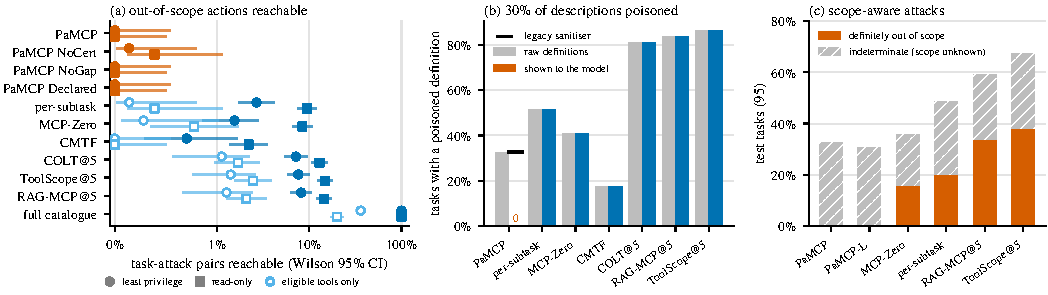
\includegraphics[width=\textwidth]{evaluation_tsc/figures/fig_sec_injection}
\caption{Injected actions: (a) reachable out-of-scope actions, (b) poisoned definitions shown to the model,
(c) scope of admitted attacks.}
\label{fig:ev-injection}
\end{figure*}

No out-of-scope action is reachable through \pamcp{}'s toolkits: 0 of 712 task--attack pairs under least privilege
and 0 of 775 under a read-only policy, against 0.7--8.1\% and 8.4--14.7\% for the published baselines
(Fig.~\ref{fig:ev-injection}a; F5, $p_{\mathrm{Holm}}<0.001$). Counting only attacks that are definitely out of
scope, no \pamcp{} toolkit admits one, against 15.8\% of the tasks for MCP-Zero, 20.0\% for per-subtask retrieval,
33.7\% for RAG-MCP and 37.9\% for ToolScope (H5: $-20.0$ points, 95\% CI $[-28.4,-12.6]$,
$p_{\mathrm{Holm}}<0.001$), although 32.6\% admit an attack whose scope the labels cannot decide. With 30\% of the
descriptions poisoned, the aliased manifest never shows an injected instruction, whereas the definitions exposed
by the baselines carry one in 17.4--86.2\% of the tasks (Fig.~\ref{fig:ev-injection}b). Moreover, 55.5\% of
\pamcp{}'s toolkits return remote content, but none of them also enables an out-of-scope action, against
3.2--22.6\% for the baselines.

\begin{table}[t]
\centering
\caption{Ablation of the gap (G), eligibility (P) and set reasoning (S).}
\label{tab:ev-factorial}
\scriptsize
\setlength{\tabcolsep}{3pt}
\begin{tabular}{@{}cccrrrrr@{}}
\toprule
G & P & S & Recall & Tokens & Joint (\%) & Reach (\%) & Abst. (\%) \\
\midrule
-- & -- & -- & 0.270 & 297 & 53.5 & 1.1 & 0.0 \\
on & -- & -- & 0.239 & 208 & 55.5 & 0.4 & 0.0 \\
-- & on & -- & 0.295 & 316 & 58.1 & 0.1 & 0.0 \\
-- & -- & on & 0.223 & 221 & 52.9 & 0.1 & 16.1 \\
on & on & -- & 0.253 & 229 & 56.8 & 0.1 & 0.0 \\
on & -- & on & 0.230 & 189 & 54.8 & 0.0 & 6.5 \\
-- & on & on & 0.183 & 193 & 55.5 & 0.0 & 20.0 \\
on & on & on & 0.181 & 176 & 56.1 & 0.0 & 10.3 \\
\midrule
\multicolumn{3}{@{}l}{Full, no backward closure} & 0.181 & 173 & 53.5 & 0.0 & 12.3 \\
\multicolumn{3}{@{}l}{Full, flow along derivations} & 0.236 & 206 & 60.6 & 0.0 & 5.8 \\
\multicolumn{3}{@{}l}{Full, no relevance term} & 0.167 & 141 & 54.8 & 0.0 & 10.3 \\
\multicolumn{3}{@{}l}{Full, no utility floor} & 0.181 & 176 & 56.1 & 0.0 & 10.3 \\
\multicolumn{3}{@{}l}{Full, no refinement} & 0.179 & 175 & 55.5 & 0.0 & 11.0 \\
\bottomrule
\end{tabular}
\end{table}

The factorial design (Table~\ref{tab:ev-factorial}) shows that each mechanism contributes. Eligibility removes
most reachable actions, and with gap analysis and set reasoning, reachability falls from 5.2\% of the tasks to none
(Shapley shares of 23\%, 35\% and 42\% for G, P and S). Gap analysis and set reasoning shrink the context from 297
to 176 tokens (main effects of $-56$ and $-67$ tokens, $p<0.001$), and the gap halves abstentions (10.3\% against
20.0\%). The price is recall (0.270 to 0.181, mainly through S), and no mechanism changes the coarse joint
feasibility. Under the labelled threat model, \pamcp{}'s mechanisms therefore jointly close the action and
metadata channels that retrieval baselines leave open.

\subsection{Scalability, Optimality and Adaptation to Registry Change}
\label{sec:ev-eff}

The last experiment addresses RQ4, discovery at a cost that scales and under registry change, together with the
optimality of the composition studied under RQ3. It measures what discovery costs, how close the composition is
to the optimum, and whether the engine keeps its guarantees under change. The engine is compared with eager
materialisation of the risk relation, with the greedy regime and an integer program (HiGHS) written independently
of the engine, with full rebuilds and cache flushes, and with cold discovery without experience reuse.

\begin{figure*}[t]
\centering
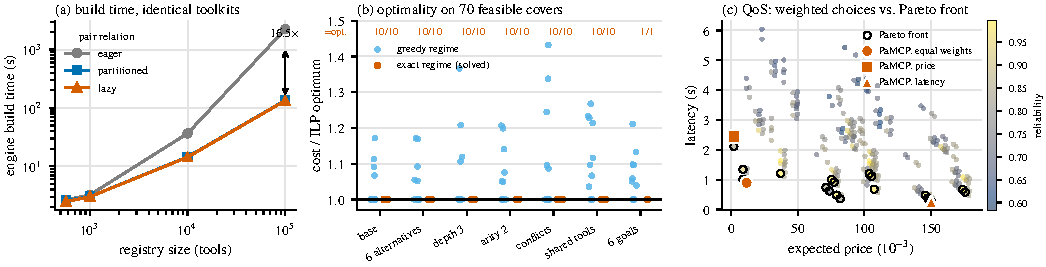
\includegraphics[width=\textwidth]{evaluation_tsc/figures/fig_tsc_eff}
\caption{Efficiency: (a) engine build time by pair-relation mode, (b) cost relative to the ILP optimum, (c) QoS
choices and Pareto front.}
\label{fig:ev-eff}
\end{figure*}

On the real registry, a request takes 49\,ms at the median (eligibility 0.08\,ms, against 12\,ms for RAG-MCP's
single dense ranking) and 2.7\,s at $10^5$ cloned tools. Deciding the pairwise risk relation lazily or by effect
class gives identical toolkits on all test tasks and builds the engine at $10^5$ tools in 133--134\,s instead of
2,224\,s, 16.5 times faster with near-linear growth (Fig.~\ref{fig:ev-eff}a); on heterogeneous registries of
$10^4$ tools, the lazy build takes 4.6--5.9\,s. Wherever the exact search finishes, it returns the ILP optimum (61
of 61 solved instances across alternatives, depth, arity, conflicts and shared tools) and recognises all ten
infeasible instances, while the greedy regime is 4.4--12.6\% above the optimum on average
(Fig.~\ref{fig:ev-eff}b); with six goals, the search exhausts its budget and falls back to greedy (6.9\% above).
When providers differ in price, latency and reliability, every equal-weight choice is Pareto-optimal and meets the
utility floor, and the weights move the choice along the front as intended (price only: 0.33$\times$ price;
latency only: 0.73$\times$ latency; Fig.~\ref{fig:ev-eff}c).

The engine also adapts to change at low cost. An incremental update takes 13.5\,ms against 4.2\,s for a rebuild,
the exact invalidation of Proposition~3 touches 1.1\% of the cached toolkits instead of all of them, and all 20
simulated rug pulls lose their evidence. Experience reuse serves 32.7\% of 300 requests without an analyst call,
with unchanged certification (82.7\% against 82.3\%) and no violation in 89 revalidation probes (removed servers,
revoked or rewritten tools, stricter principal, other model). Deterministic repair raises certification from
72.6\% to 87.4\% when counterexamples are induced. The complete engine thus scales to $10^5$ tools, composes
optimally where it searches exactly, makes Pareto-consistent QoS trade-offs and adapts to change without losing
its guarantees.

\subsection{Summary of Findings and Threats to Validity}
\label{sec:ev-threats}

\begin{table}[t]
\centering
\caption{Summary of findings (Conf.: confirmatory test, $p_{\mathrm{Holm}}$).}
\label{tab:ev-answers}
\scriptsize
\setlength{\tabcolsep}{2pt}
\begin{tabular}{@{}lp{2.85cm}p{2.95cm}l@{}}
\toprule
Aspect & Result & Best baseline & Conf. \\
\midrule
Profile & FNR $\le$3.6\% at 83--100\% coverage & self-assessment ECE 0.20--0.39 & -- \\
Eligibility & Exp@5 0\% (swap 2.3--3.9\%), Util $-3.6$ & lexical 9.9\%, MCP default 42.5\% & F4 $<$0.001 \\
Execution & labels = execution, 30/30 calls & -- (observed) & -- \\
Feasibility & strict joint 27.7\%, 1.46 tools & 5.3--14.9\%, 0.64--5.2 tools & expl. \\
Recall & recall at equal size 0.189 & 0.084--0.200 & F2 n.s. \\
Retrieval & Hit@1 (569) 41.3\% & MCP-Zero 66.7\% & F7 against \\
Security & reachable 0/712, definite 0\% & 0.7--8.1\%, 15.8--37.9\% & F5, H5 $<$0.001 \\
Scaling & build 16.5$\times$ faster; =ILP 61/61 & eager 2,224\,s; greedy +4--13\% & -- \\
Evolution & update 13.5\,ms; reuse 32.7\% & rebuild 4.2\,s; cold & -- \\
\bottomrule
\end{tabular}
\end{table}

\begin{table}[t]
\centering
\caption{Confirmatory comparisons (Holm-corrected; $\Delta$: \pamcp{} minus comparator, in points, tokens for F6).}
\label{tab:ev-family}
\scriptsize
\setlength{\tabcolsep}{2.2pt}
\begin{tabular}{@{}llrlll@{}}
\toprule
 & Comparison & $\Delta$ & 95\% CI & $p_{\mathrm{Holm}}$ & Verdict \\
\midrule
F1 & Group recall vs per-subtask (non-inf., 0.05) & -8.0 & [-16.6, +0.2] & 1.000 & not shown \\
F2 & Size-matched recall vs RAG-MCP & +6.0 & [-1.6, +13.7] & 0.397 & n.s. \\
F3 & Joint feasibility vs per-subtask (elig.) & +4.3 & [-8.5, +18.1] & 1.000 & n.s. \\
F4 & Exp@5 verified vs lexical & -9.9 & [-13.9, -6.6] & $<$0.001 & supports \\
F5 & Reachable attacks vs per-subtask & -2.7 & [-3.9, -1.5] & $<$0.001 & supports \\
F6 & Tokens, full vs NoGap & -16.7 & [-34.6, +1.0] & 0.269 & n.s. \\
F7 & Hit@1 goal contract vs raw RRF (569) & -15.7 & [-21.3, -10.0] & $<$0.001 & against \\
\midrule
H1 & Hit@1 PaMCP-L vs tuned BM25 (569) & +0.3 & [-8.9, +8.8] & 1.000 & n.s. \\
H2 & Hit@1 PaMCP-L vs Eq. (5) (569) & +11.7 & [+3.0, +22.6] & 0.070 & n.s. \\
H3 & Group recall PaMCP-L vs per-subtask (non-inf.) & -8.8 & [-17.6, -0.5] & 1.000 & not shown \\
H4 & Strict joint feas. vs per-subtask (elig.) & +7.4 & [+0.0, +14.9] & 0.277 & n.s. \\
H5 & Definite out-of-scope vs per-subtask & -20.0 & [-28.4, -12.6] & $<$0.001 & supports \\
\bottomrule
\end{tabular}
\end{table}

Table~\ref{tab:ev-answers} summarises the findings for RQ1--RQ4, and Table~\ref{tab:ev-family} the confirmatory
tests. All confirmatory tests on safety (F4, F5 and H5) favour \pamcp{} at $p_{\mathrm{Holm}}<0.001$; the tests on
recall and retrieval do not, and the feasibility advantage under the strict evaluator is exploratory.

These findings are subject to several threats to validity. Effects, types and feasibility are scored against LLM
labels; execution confirms them on 30 calls of six non-adversarial reference servers, and the label swap bounds
the effect of labeller disagreement but not of errors shared by one model family. Reachability is decided offline:
whether an agent follows an injected instruction, and end-to-end task success, require executing the toolkits,
which this study did not do. The baselines are adaptations sharing a TF-IDF and SVD encoder, all tuned on the same
development split; larger registries are cloned or generated, and QoS data are synthetic. Executed compositions
over isolated and adversarial servers, human annotation of a stratified tool sample and reproductions of the
baselines with their original encoders are the natural next steps, and the released artifact supports each of
them.
; needs graphicx, booktabs, amsmath, url.
% Generated by paper/package_overleaf.py from paper/sections/evaluation_tsc.tex
% (repository msellamiTN/taas-provenance-discovery, branch research/pamcp-final-evaluation).
\providecommand{\pamcp}{PaMCP}
\section{Experimental Evaluation}
\label{sec:ev}

This section evaluates \pamcp{} against the strongest baselines we could configure. Every result is labelled by
its evidence class: \emph{measured} from the running system, \emph{observed} from executed servers,
\emph{labelled} against reference labels, or \emph{simulated} under stated assumptions; the main comparisons are
confirmed with pre-registered tests.

\subsection{Datasets, Baselines and Evaluation Protocol}
\label{sec:ev-setup}

\begin{table}[t]
\centering
\caption{Datasets and compared methods.}
\label{tab:ev-setup}
\scriptsize
\setlength{\tabcolsep}{2.5pt}
\begin{tabular}{@{}p{2.3cm}p{5.65cm}@{}}
\toprule
\multicolumn{2}{@{}l}{\emph{Data}} \\
Registry & 569 tools, 76 servers (LiveMCPTool \cite{mo2025livemcpbench} + MCPToolBench++ \cite{fan2025mcptoolbench}); 44 annotated \\
Multi-step tasks & 95 LiveMCPBench tasks (test); 60 development prompts \\
Single-tool requests & 60 development / 300 test (50 per category, 66 targets) \\
Calibration suite & 432 items: 6 operations, $n\in\{10,40,160,640\}$, en/fr, noise, context; 264 cal.\ / 168 test \\
Executed servers & 6 MCP reference servers, 37 registry tools \\
Synthetic & cloned and heterogeneous registries ($10^3$--$10^5$); 80 cover and 120 QoS instances \\
\midrule
\multicolumn{2}{@{}l}{\emph{Baselines (adapted to one registry, one encoder; tuned on the development split)}} \\
RAG-MCP \cite{gan2025ragmcp} & dense top-$k$ over the request \\
MCP-Zero \cite{fei2025mcpzero} & model-written requests, server routing \\
COLT \cite{qu2024colt} & collaborative graph of 450 training queries \\
ToolScope \cite{liu2026toolscope} & LLM-confirmed tool merging, subquery retrieval \\
CMTF \cite{suresh2026cmtf} & typed-state search, one tool per step \\
BM25, RRF, per-subtask & lexical, fused, one tool per analyst subgoal \\
\midrule
\multicolumn{2}{@{}l}{\emph{Ablations of \pamcp{}}} \\
G, P, S & gap (Alg.~1), eligibility (Sec.~5), set reasoning + certificate (Sec.~6), $2^3$ design \\
\pamcp{}-L & relevance-first ranking selected on the development split \\
\bottomrule
\end{tabular}
\end{table}

\begin{table}[t]
\centering
\caption{Experimental parameters (defaults in bold).}
\label{tab:ev-params}
\scriptsize
\setlength{\tabcolsep}{2.5pt}
\begin{tabular}{@{}lp{4.3cm}@{}}
\toprule
Parameter & Values \\
\midrule
Profile threshold $\tau$ / risk target & 0.6, 0.75, \textbf{0.9} / 0.05, 0.10 \\
Forging servers $\delta$; false accepts $\varphi$ & 0--0.3 (5 seeds); 0--0.2, \textbf{0.05} \\
Probe coverage $\kappa$; trust $\ell_{\min}$ & 0.25--\textbf{1}; 0.2--0.95, \textbf{0.65} \\
Candidate budget $K$; size matching & 1, 5, \textbf{10}, 20, 40; equal $|K|$ \\
Poisoned descriptions; policies & 10\%, 30\%; least privilege, read-only \\
Registry size; pair relation & 569--$10^5$; eager, partitioned, \textbf{lazy} \\
Cost weights; utility floor $u_{\min}$ & 0, 0.25, \textbf{0.5}, 1; 0--0.9 \\
\bottomrule
\end{tabular}
\end{table}

Table~\ref{tab:ev-setup} lists the data and the compared methods, and Table~\ref{tab:ev-params} the parameters
varied across the experiments. Effects and types are scored against blind labels $J_B$ (Claude Opus), which are
not used to simulate evidence; the simulated verifier uses labels $J_A$ (Claude Sonnet), and we report the
swapped direction and executed servers to remove the dependency between the two. All LLM outputs were recorded
once and are replayed, and every method, including \pamcp{}, was configured on the development split only.
Request-level metrics are resampled with target tools as clusters and task-level metrics with tasks; paired tests
are sign-flip permutation tests, and proportions use Wilson intervals (95\%). Two confirmatory families (F1--F7,
H1--H5) were fixed before the data they test and are Holm-corrected. Code, records, manifests and a notebook that
re-runs every experiment on a CPU are public.\footnote{\url{https://github.com/msellamiTN/taas-provenance-discovery},
branch \texttt{research/pamcp-final-evaluation}; guide in \texttt{docs/REPRODUCIBILITY.md}.}

\subsection{Measured Model Profiles for Model-Conditioned Discovery}
\label{sec:ev-rq1}

The first experiment addresses RQ1, the conditioning of discovery on the deployed model. It tests whether a
measured profile $\rho_{\mathrm{LLM}}$ decides reliably which operations the deployed model keeps, and whether the
gap responds to the model and to the input. Three models answer the calibration suite by reading only, after
stating for each cell their probability of success; $\tau$ is chosen on the calibration split for a risk target
and evaluated on held-out items (measured). The measured profile is compared with two baselines, the model's own
self-assessment and the earlier 64-item profile.

\begin{table}[t]
\centering
\caption{Calibration of the model profile (Cov.: operations kept native; FNR: false-native rate).}
\label{tab:ev-calibration}
\scriptsize
\setlength{\tabcolsep}{2.2pt}
\begin{tabular}{@{}lrcrrrrrrrr@{}}
\toprule
 & & & & \multicolumn{2}{c}{Self-assess.} & \multicolumn{3}{c}{Measured, risk 5\%} & \multicolumn{2}{c}{64-item} \\
\cmidrule(lr){5-6}\cmidrule(lr){7-9}\cmidrule(l){10-11}
Model & $n$ & Accuracy (\%) & $n{=}640$ & ECE & Brier & $\tau$ & Cov. & FNR & Cov. & FNR \\
\midrule
Haiku & 432 & 86.1 [82.5, 89.1] & 67 & 0.39 & 0.30 & 0.21 & 83 & 3.6 & 21 & 0.0 \\
Sonnet & 432 & 91.4 [88.4, 93.7] & 62 & 0.20 & 0.11 & 0.42 & 90 & 3.3 & 26 & 4.5 \\
Opus & 387 & 100.0 [99.0, 100.0] & 100 & 0.38 & 0.20 & 0.90 & 100 & 0.0 & -- & -- \\
\bottomrule
\end{tabular}
\end{table}

\begin{figure*}[t]
\centering
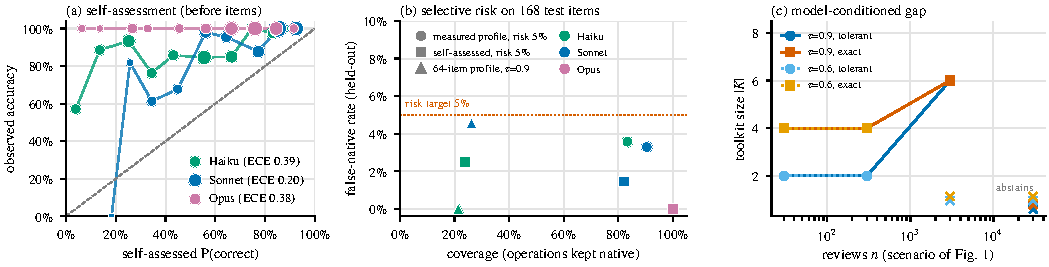
\includegraphics[width=\textwidth]{evaluation_tsc/figures/fig_rq1_profile}
\caption{Model profile: (a) self-assessment reliability, (b) coverage versus false-native rate, (c) toolkit size
versus input size (crosses: abstentions).}
\label{fig:ev-profile}
\end{figure*}

Capability boundaries differ by model and by operation (Table~\ref{tab:ev-calibration}). Haiku fails counting
from $n=40$, Sonnet loses joins as they grow, and both fail approximate sums over 640 values, whereas Opus answers
all 387 items it was given. With the measured profile and a 5\% risk target, the held-out false-native rate stays
within the target for every model (3.6\%, 3.3\% and 0.0\%) while 83--100\% of the operations remain with the model
(Fig.~\ref{fig:ev-profile}b). Both baselines fail. Self-assessment is miscalibrated for every model (ECE
0.20--0.39, all underconfident; Fig.~\ref{fig:ev-profile}a), and the 64-item profile keeps only 21--26\% of the
operations native, sending most correctly performed work to tools. The gap, in turn, behaves as designed
(Fig.~\ref{fig:ev-profile}c): two tools suffice for 30 or 300 reviews and six for 3,000, and the engine abstains
rather than return an unsupported toolkit at 30,000; without gap analysis, it abstains in every setting. On the
test tasks, the profile overrules 9.4\% of the analyst's claims that an operation is native. A measured,
risk-targeted profile therefore makes model conditioning reliable, and neither self-assessment nor a small profile
can replace it.

\subsection{Evidence-Based Eligibility under Forged and Imperfect Metadata}
\label{sec:ev-rq2}

The second experiment addresses RQ2, the restriction of discovery to tools whose safety-relevant behaviour is
evidenced. It measures whether provenance-sound eligibility (P) keeps unsafe tools away from the model, and at what
cost, under a read-only policy over 273 requests with read-only gold tools. Exp@5 is the share of requests whose
top five contain a tool that is not read-only under $J_B$, and Util@5 the share whose top five contain a gold
tool; forgery and verifier errors are simulated. Verified evidence is compared with four encodings of the
policy, namely no filter, MCP's default (annotations displayed, not enforced), annotations as a closed world, and
lexical cues, each combined with \pamcp{}'s retrieval and with MCP-Zero.

\begin{table}[t]
\centering
\caption{Exposure and utility of read-only policy encodings (\%).}
\label{tab:ev-encodings}
\scriptsize
\setlength{\tabcolsep}{2.2pt}
\begin{tabular}{@{}lrrrrrrr@{}}
\toprule
 & & & \multicolumn{2}{c}{\pamcp{} retr.} & \multicolumn{2}{c}{MCP-Zero} & $\delta{=}0.2$ \\
\cmidrule(lr){4-5}\cmidrule(lr){6-7}\cmidrule(l){8-8}
Encoding & Elig. & Unsafe & Exp@5 & Util@5 & Exp@5 & Util@5 & Exp@5 \\
\midrule
no filter & 100.0 & 120 & 42.5 & 49.8 & 26.4 & 76.6 & 43.7 \\
MCP default (display only) & 100.0 & 120 & 42.5 & 49.8 & 26.4 & 76.6 & 43.7 \\
closed-world annotations & 7.7 & 1 & 31.5 & 0.4 & 0.0 & 0.4 & 58.7 \\
lexical cues & 67.8 & 21 & 9.9 & 41.0 & 12.5 & 65.6 & 8.8 \\
verified evidence (P) & 77.0 & 0 & 0.0 & 46.2 & 0.0 & 72.2 & 5.5 \\
observed + lexical fallback & 77.0 & 0 & 0.0 & 46.2 & 0.0 & 72.2 & 5.5 \\
attested only & 26.4 & 0 & 0.0 & 16.5 & 0.0 & 18.3 & 5.8 \\
\bottomrule
\end{tabular}
\end{table}

\begin{figure*}[t]
\centering
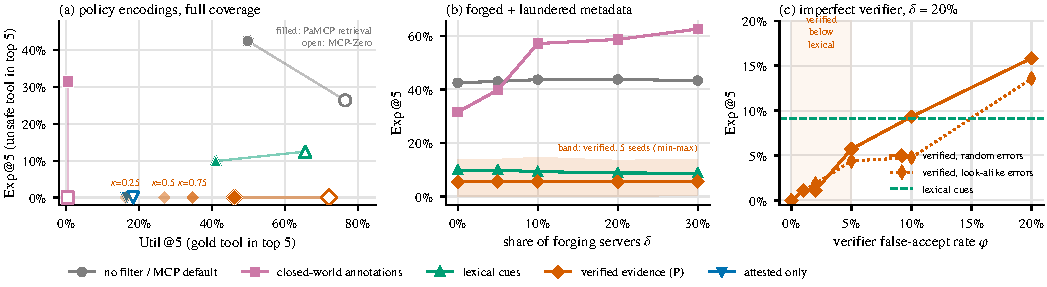
\includegraphics[width=\textwidth]{evaluation_tsc/figures/fig_rq2_exposure}
\caption{Exposure to unsafe tools: (a) policy encodings, (b) forged metadata, (c) verifier false accepts.}
\label{fig:ev-exposure}
\end{figure*}

Every baseline encoding exposes unsafe tools (Table~\ref{tab:ev-encodings}): 42.5\% of the requests without a
filter or under MCP's default, 31.5\% with annotations as a closed world (whose utility falls to 0.4\%), and 9.9\%
with lexical cues. Verified evidence admits none of the 120 unsafe tools, keeps 77\% of the registry eligible and
costs 3.6 utility points (4.4 for MCP-Zero); its difference to lexical cues is confirmatory (F4: $-9.9$ points,
$p_{\mathrm{Holm}}<0.001$). Under forgery, the closed-world reading collapses (31.5\% to 62.6\% exposure at
$\delta=0.3$), while verified evidence stays at 5.4--5.6\% for every $\delta$ with a 5\% false-accept rate
(Fig.~\ref{fig:ev-exposure}b) and remains below lexical cues up to $\varphi=5\%$ (10\% for look-alike errors;
Fig.~\ref{fig:ev-exposure}c).

\begin{figure*}[t]
\centering
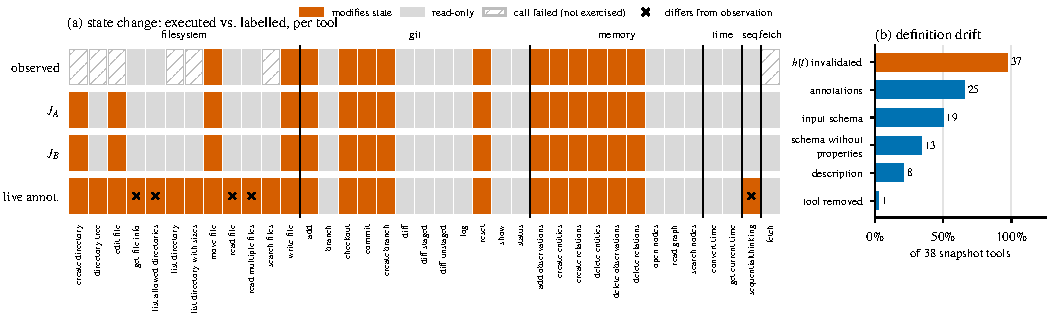
\includegraphics[width=\textwidth]{evaluation_tsc/figures/fig_rq2_observed}
\caption{Executed reference servers: (a) observed and labelled state changes, (b) definition drift since the
benchmark snapshot.}
\label{fig:ev-observed}
\end{figure*}

Three further checks remove the dependency on how the labels were built. First, with the verifier simulated from
$J_B$ and scored on $J_A$, exposure is 2.3--3.9\% across \pamcp{}, RAG-MCP, MCP-Zero and ToolScope, a quarter to
two fifths of the exposure left by lexical cues. Second, when the six MCP reference servers are executed under
system-call tracing (observed; Fig.~\ref{fig:ev-observed}), both labellings agree with all 30 completed calls: none
of the 13 tools observed to change state is labelled read-only (Wilson upper bound 22.8\%). Third, every one of the
37 surviving definitions changed since the benchmark snapshot, so evidence not bound to $h(t)$, as \pamcp{} binds
it, would have been stale. Eligibility based on verified, hash-bound evidence thus removes the exposure that
published metadata leaves, degrades in proportion to verifier error, and does not depend on the reference labels.

\subsection{Compactness and Joint Feasibility of Certified Toolkits}
\label{sec:ev-rq3}

The third experiment addresses RQ3, the return of a small toolkit whose interfaces, effects and flows are
certified jointly before any call. It examines whether set-level reasoning returns smaller toolkits that are
jointly feasible more often than retrieval on the 94 test tasks, against RAG-MCP, COLT and ToolScope (top five),
MCP-Zero, CMTF and per-subtask retrieval, each also restricted to eligible tools. Group recall is measured against
benchmark gold (measured), and joint feasibility is decided by two evaluators written independently of the
certificate: a coarse one, and a strict one that also checks domains, cardinality, schema-required inputs and
egress of private data (labelled). On ten hand-built cases with known answers, the strict evaluator decides 7
correctly and the coarse one 2.

\begin{table}[t]
\centering
\caption{Toolkit size, recall and joint feasibility on the 94 test tasks.}
\label{tab:ev-sets}
\scriptsize
\setlength{\tabcolsep}{2.1pt}
\begin{tabular}{@{}lrrlrrr@{}}
\toprule
 & & & & \multicolumn{2}{c}{Joint feas. (\%)} & \\
\cmidrule(lr){5-6}
Method & $|K|$ & Tok. & Group recall [CI] & coarse & strict & Abst. \\
\midrule
\pamcp{} ($K{=}10$) & 1.46 & 198 & 0.174 [0.12, 0.23] & 67.0 & 27.7 & 7.4 \\
\pamcp{}-L & 1.22 & 146 & 0.161 & 54.7 & 15.8 & 9.5 \\
\pamcp{} NoCert & -- & -- & -- & 59.6 & 13.8 & 0.0 \\
Per-subtask (elig.) & 2.59 & 346 & 0.249 [0.19, 0.32] & 62.8 & 8.5 & -- \\
RAG-MCP@5 (elig.) & 5.00 & 1244 & 0.293 [0.22, 0.37] & 60.6 & 5.3 & -- \\
COLT@5 (elig.) & 5.00 & 1094 & 0.295 [0.23, 0.37] & 59.6 & 8.5 & -- \\
ToolScope@5 (elig.) & 5.20 & 976 & 0.361 [0.29, 0.44] & 73.4 & 11.7 & -- \\
MCP-Zero (elig.) & 1.76 & 250 & 0.227 [0.17, 0.29] & 57.4 & 11.7 & -- \\
CMTF (elig.) & 0.64 & 105 & 0.072 [0.04, 0.11] & 25.5 & 14.9 & -- \\
RAG-MCP@5 (published) & 5.00 & 1244 & 0.293 [0.22, 0.37] & 48.9 & 5.3 & -- \\
\bottomrule
\end{tabular}
\end{table}

\begin{figure*}[t]
\centering
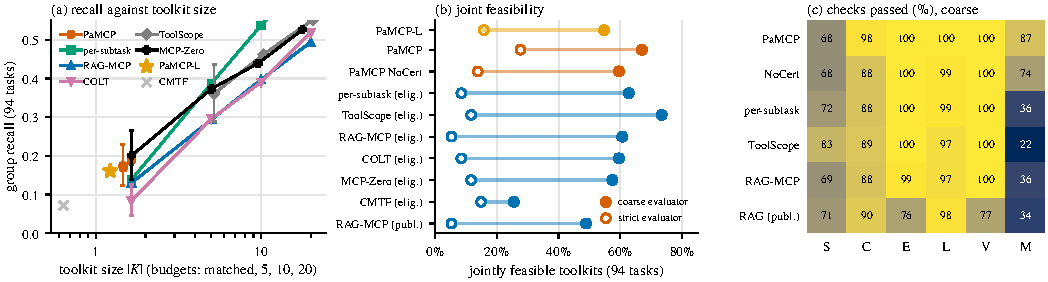
\includegraphics[width=\textwidth]{evaluation_tsc/figures/fig_rq3_sets}
\caption{Toolkit quality: (a) recall versus toolkit size, (b) joint feasibility, (c) certificate checks passed
(S goals, C inputs, E effects, L flows, V evidence, M minimality).}
\label{fig:ev-sets}
\end{figure*}

\pamcp{} returns the smallest toolkits apart from CMTF, with 1.46 tools and 198 tokens against 5 tools and
976--1,244 tokens for the top-five retrievers (Table~\ref{tab:ev-sets}), and it certifies 92.6\% of the tasks,
abstaining with a counterexample on the rest. Under the strict evaluator, its toolkits are jointly feasible in
27.7\% of the tasks, 1.9 to 5.2 times as often as every baseline restricted to eligible tools (5.3--14.9\%) and
twice as often as without certification (13.8\%; Fig.~\ref{fig:ev-sets}b). Certification acts through obtainable
inputs and minimality (C 88\% to 98\%, M 74\% to 87\%, against 22--36\% for the top-five retrievers;
Fig.~\ref{fig:ev-sets}c). At equal size, \pamcp{} reaches more gold steps than RAG-MCP, per-subtask retrieval and
COLT (0.189 against 0.130, 0.138 and 0.084; F2 not significant after correction), whereas retrievers that expose
three to four times more tools reach more (0.249--0.361; non-inferiority to per-subtask retrieval, F1, not shown).
\pamcp{} thus trades breadth for certified compactness.

\begin{table}[t]
\centering
\caption{Single-tool retrieval accuracy on the 300 test requests.}
\label{tab:ev-retrieval}
\scriptsize
\setlength{\tabcolsep}{2.4pt}
\begin{tabular}{@{}lrrrrrr@{}}
\toprule
 & 81 tools & \multicolumn{5}{c}{569 tools} \\
\cmidrule(lr){2-2}\cmidrule(l){3-7}
Method & Hit@1 & Hit@1 [CI] & Hit@3 & Hit@5 & MRR & nDCG \\
\midrule
BM25 & 52.7 & 41.0 [26, 60] & 57.3 & 63.7 & 0.503 & 0.543 \\
RAG-MCP (dense) & 49.7 & 37.3 [22, 56] & 50.0 & 54.3 & 0.451 & 0.492 \\
RRF fusion & 54.3 & 38.7 [23, 57] & 54.7 & 61.3 & 0.481 & 0.525 \\
MCP-Zero & 68.0 & 66.7 [49, 80] & 80.0 & 85.7 & 0.743 & 0.775 \\
COLT & 49.7 & 37.3 [22, 56] & 50.0 & 54.3 & 0.451 & 0.492 \\
ToolScope & 53.0 & 41.0 [26, 60] & 58.3 & 63.7 & 0.504 & 0.543 \\
CMTF & 58.7 & 32.7 [19, 49] & 47.0 & 54.7 & 0.428 & 0.488 \\
PaMCP (Eq. 5) & 61.0 & 29.7 [16, 47] & 45.7 & 53.7 & 0.400 & 0.461 \\
PaMCP-L & 72.0 & 41.3 [25, 60] & 61.3 & 69.3 & 0.536 & 0.603 \\
PaMCP, oracle types (diag.) & 71.7 & 58.3 [38, 74] & 75.3 & 81.3 & 0.680 & 0.728 \\
\bottomrule
\end{tabular}
\end{table}

Single-tool retrieval, in contrast, is not where \pamcp{} gains (Table~\ref{tab:ev-retrieval}). Over 81 tools, its
relevance-first ranking is the most accurate (72.0\% Hit@1, against 68.0\% for MCP-Zero), but over the full
registry MCP-Zero leads (66.7\%), \pamcp{}-L ties tuned BM25 (41.3\% against 41.0\%; H1 n.s.), and the structural
ranking of Eq.~(5) falls to 29.7\% (F7 against \pamcp{}), because types agree with $J_B$ on 78.9\% of output kinds
but only on 35.7\% of domains. With correct types, the same ranking reaches 58.3\%, above every baseline except
MCP-Zero, which locates the limit in the typing rather than in the composition. Set-level reasoning therefore
yields the most compact and most often jointly feasible toolkits, while finding more tools requires better typing
or a larger budget.

\subsection{Resistance to Injected Actions and Contribution of the Mechanisms}
\label{sec:ev-sec}

The fourth experiment combines RQ2 and RQ3. It measures whether the exposed
toolkit limits what an injected instruction could achieve, and which mechanism is responsible. For 155 tasks and
each attack class outside the task's needs, an attack is reachable if the toolkit can realise it under $J_B$
(labelled, offline). Poisoning places a canary in the description, name or argument keys of 10--30\% of the tools,
and we scan what each method shows the model; the mechanisms are varied in a $2^3$ design with Shapley
attribution.

\begin{figure*}[t]
\centering
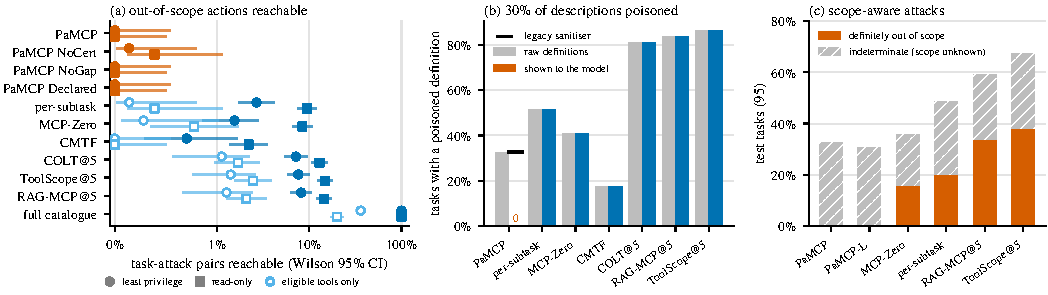
\includegraphics[width=\textwidth]{evaluation_tsc/figures/fig_sec_injection}
\caption{Injected actions: (a) reachable out-of-scope actions, (b) poisoned definitions shown to the model,
(c) scope of admitted attacks.}
\label{fig:ev-injection}
\end{figure*}

No out-of-scope action is reachable through \pamcp{}'s toolkits: 0 of 712 task--attack pairs under least privilege
and 0 of 775 under a read-only policy, against 0.7--8.1\% and 8.4--14.7\% for the published baselines
(Fig.~\ref{fig:ev-injection}a; F5, $p_{\mathrm{Holm}}<0.001$). Counting only attacks that are definitely out of
scope, no \pamcp{} toolkit admits one, against 15.8\% of the tasks for MCP-Zero, 20.0\% for per-subtask retrieval,
33.7\% for RAG-MCP and 37.9\% for ToolScope (H5: $-20.0$ points, 95\% CI $[-28.4,-12.6]$,
$p_{\mathrm{Holm}}<0.001$), although 32.6\% admit an attack whose scope the labels cannot decide. With 30\% of the
descriptions poisoned, the aliased manifest never shows an injected instruction, whereas the definitions exposed
by the baselines carry one in 17.4--86.2\% of the tasks (Fig.~\ref{fig:ev-injection}b). Moreover, 55.5\% of
\pamcp{}'s toolkits return remote content, but none of them also enables an out-of-scope action, against
3.2--22.6\% for the baselines.

\begin{table}[t]
\centering
\caption{Ablation of the gap (G), eligibility (P) and set reasoning (S).}
\label{tab:ev-factorial}
\scriptsize
\setlength{\tabcolsep}{3pt}
\begin{tabular}{@{}cccrrrrr@{}}
\toprule
G & P & S & Recall & Tokens & Joint (\%) & Reach (\%) & Abst. (\%) \\
\midrule
-- & -- & -- & 0.270 & 297 & 53.5 & 1.1 & 0.0 \\
on & -- & -- & 0.239 & 208 & 55.5 & 0.4 & 0.0 \\
-- & on & -- & 0.295 & 316 & 58.1 & 0.1 & 0.0 \\
-- & -- & on & 0.223 & 221 & 52.9 & 0.1 & 16.1 \\
on & on & -- & 0.253 & 229 & 56.8 & 0.1 & 0.0 \\
on & -- & on & 0.230 & 189 & 54.8 & 0.0 & 6.5 \\
-- & on & on & 0.183 & 193 & 55.5 & 0.0 & 20.0 \\
on & on & on & 0.181 & 176 & 56.1 & 0.0 & 10.3 \\
\midrule
\multicolumn{3}{@{}l}{Full, no backward closure} & 0.181 & 173 & 53.5 & 0.0 & 12.3 \\
\multicolumn{3}{@{}l}{Full, flow along derivations} & 0.236 & 206 & 60.6 & 0.0 & 5.8 \\
\multicolumn{3}{@{}l}{Full, no relevance term} & 0.167 & 141 & 54.8 & 0.0 & 10.3 \\
\multicolumn{3}{@{}l}{Full, no utility floor} & 0.181 & 176 & 56.1 & 0.0 & 10.3 \\
\multicolumn{3}{@{}l}{Full, no refinement} & 0.179 & 175 & 55.5 & 0.0 & 11.0 \\
\bottomrule
\end{tabular}
\end{table}

The factorial design (Table~\ref{tab:ev-factorial}) shows that each mechanism contributes. Eligibility removes
most reachable actions, and with gap analysis and set reasoning, reachability falls from 5.2\% of the tasks to none
(Shapley shares of 23\%, 35\% and 42\% for G, P and S). Gap analysis and set reasoning shrink the context from 297
to 176 tokens (main effects of $-56$ and $-67$ tokens, $p<0.001$), and the gap halves abstentions (10.3\% against
20.0\%). The price is recall (0.270 to 0.181, mainly through S), and no mechanism changes the coarse joint
feasibility. Under the labelled threat model, \pamcp{}'s mechanisms therefore jointly close the action and
metadata channels that retrieval baselines leave open.

\subsection{Scalability, Optimality and Adaptation to Registry Change}
\label{sec:ev-eff}

The last experiment addresses RQ4, discovery at a cost that scales and under registry change, together with the
optimality of the composition studied under RQ3. It measures what discovery costs, how close the composition is
to the optimum, and whether the engine keeps its guarantees under change. The engine is compared with eager
materialisation of the risk relation, with the greedy regime and an integer program (HiGHS) written independently
of the engine, with full rebuilds and cache flushes, and with cold discovery without experience reuse.

\begin{figure*}[t]
\centering
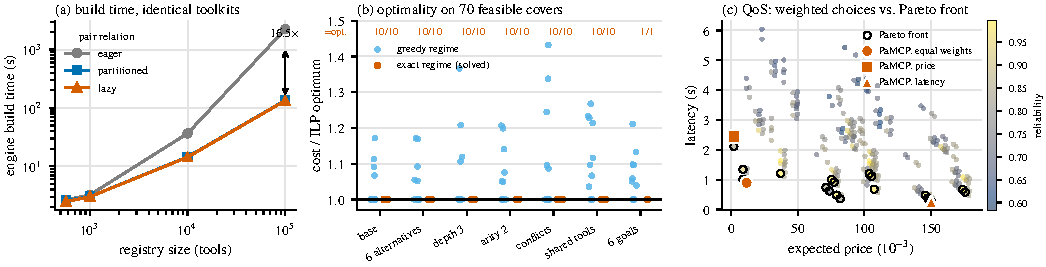
\includegraphics[width=\textwidth]{evaluation_tsc/figures/fig_tsc_eff}
\caption{Efficiency: (a) engine build time by pair-relation mode, (b) cost relative to the ILP optimum, (c) QoS
choices and Pareto front.}
\label{fig:ev-eff}
\end{figure*}

On the real registry, a request takes 49\,ms at the median (eligibility 0.08\,ms, against 12\,ms for RAG-MCP's
single dense ranking) and 2.7\,s at $10^5$ cloned tools. Deciding the pairwise risk relation lazily or by effect
class gives identical toolkits on all test tasks and builds the engine at $10^5$ tools in 133--134\,s instead of
2,224\,s, 16.5 times faster with near-linear growth (Fig.~\ref{fig:ev-eff}a); on heterogeneous registries of
$10^4$ tools, the lazy build takes 4.6--5.9\,s. Wherever the exact search finishes, it returns the ILP optimum (61
of 61 solved instances across alternatives, depth, arity, conflicts and shared tools) and recognises all ten
infeasible instances, while the greedy regime is 4.4--12.6\% above the optimum on average
(Fig.~\ref{fig:ev-eff}b); with six goals, the search exhausts its budget and falls back to greedy (6.9\% above).
When providers differ in price, latency and reliability, every equal-weight choice is Pareto-optimal and meets the
utility floor, and the weights move the choice along the front as intended (price only: 0.33$\times$ price;
latency only: 0.73$\times$ latency; Fig.~\ref{fig:ev-eff}c).

The engine also adapts to change at low cost. An incremental update takes 13.5\,ms against 4.2\,s for a rebuild,
the exact invalidation of Proposition~3 touches 1.1\% of the cached toolkits instead of all of them, and all 20
simulated rug pulls lose their evidence. Experience reuse serves 32.7\% of 300 requests without an analyst call,
with unchanged certification (82.7\% against 82.3\%) and no violation in 89 revalidation probes (removed servers,
revoked or rewritten tools, stricter principal, other model). Deterministic repair raises certification from
72.6\% to 87.4\% when counterexamples are induced. The complete engine thus scales to $10^5$ tools, composes
optimally where it searches exactly, makes Pareto-consistent QoS trade-offs and adapts to change without losing
its guarantees.

\subsection{Summary of Findings and Threats to Validity}
\label{sec:ev-threats}

\begin{table}[t]
\centering
\caption{Summary of findings (Conf.: confirmatory test, $p_{\mathrm{Holm}}$).}
\label{tab:ev-answers}
\scriptsize
\setlength{\tabcolsep}{2pt}
\begin{tabular}{@{}lp{2.85cm}p{2.95cm}l@{}}
\toprule
Aspect & Result & Best baseline & Conf. \\
\midrule
Profile & FNR $\le$3.6\% at 83--100\% coverage & self-assessment ECE 0.20--0.39 & -- \\
Eligibility & Exp@5 0\% (swap 2.3--3.9\%), Util $-3.6$ & lexical 9.9\%, MCP default 42.5\% & F4 $<$0.001 \\
Execution & labels = execution, 30/30 calls & -- (observed) & -- \\
Feasibility & strict joint 27.7\%, 1.46 tools & 5.3--14.9\%, 0.64--5.2 tools & expl. \\
Recall & recall at equal size 0.189 & 0.084--0.200 & F2 n.s. \\
Retrieval & Hit@1 (569) 41.3\% & MCP-Zero 66.7\% & F7 against \\
Security & reachable 0/712, definite 0\% & 0.7--8.1\%, 15.8--37.9\% & F5, H5 $<$0.001 \\
Scaling & build 16.5$\times$ faster; =ILP 61/61 & eager 2,224\,s; greedy +4--13\% & -- \\
Evolution & update 13.5\,ms; reuse 32.7\% & rebuild 4.2\,s; cold & -- \\
\bottomrule
\end{tabular}
\end{table}

\begin{table}[t]
\centering
\caption{Confirmatory comparisons (Holm-corrected; $\Delta$: \pamcp{} minus comparator, in points, tokens for F6).}
\label{tab:ev-family}
\scriptsize
\setlength{\tabcolsep}{2.2pt}
\begin{tabular}{@{}llrlll@{}}
\toprule
 & Comparison & $\Delta$ & 95\% CI & $p_{\mathrm{Holm}}$ & Verdict \\
\midrule
F1 & Group recall vs per-subtask (non-inf., 0.05) & -8.0 & [-16.6, +0.2] & 1.000 & not shown \\
F2 & Size-matched recall vs RAG-MCP & +6.0 & [-1.6, +13.7] & 0.397 & n.s. \\
F3 & Joint feasibility vs per-subtask (elig.) & +4.3 & [-8.5, +18.1] & 1.000 & n.s. \\
F4 & Exp@5 verified vs lexical & -9.9 & [-13.9, -6.6] & $<$0.001 & supports \\
F5 & Reachable attacks vs per-subtask & -2.7 & [-3.9, -1.5] & $<$0.001 & supports \\
F6 & Tokens, full vs NoGap & -16.7 & [-34.6, +1.0] & 0.269 & n.s. \\
F7 & Hit@1 goal contract vs raw RRF (569) & -15.7 & [-21.3, -10.0] & $<$0.001 & against \\
\midrule
H1 & Hit@1 PaMCP-L vs tuned BM25 (569) & +0.3 & [-8.9, +8.8] & 1.000 & n.s. \\
H2 & Hit@1 PaMCP-L vs Eq. (5) (569) & +11.7 & [+3.0, +22.6] & 0.070 & n.s. \\
H3 & Group recall PaMCP-L vs per-subtask (non-inf.) & -8.8 & [-17.6, -0.5] & 1.000 & not shown \\
H4 & Strict joint feas. vs per-subtask (elig.) & +7.4 & [+0.0, +14.9] & 0.277 & n.s. \\
H5 & Definite out-of-scope vs per-subtask & -20.0 & [-28.4, -12.6] & $<$0.001 & supports \\
\bottomrule
\end{tabular}
\end{table}

Table~\ref{tab:ev-answers} summarises the findings for RQ1--RQ4, and Table~\ref{tab:ev-family} the confirmatory
tests. All confirmatory tests on safety (F4, F5 and H5) favour \pamcp{} at $p_{\mathrm{Holm}}<0.001$; the tests on
recall and retrieval do not, and the feasibility advantage under the strict evaluator is exploratory.

These findings are subject to several threats to validity. Effects, types and feasibility are scored against LLM
labels; execution confirms them on 30 calls of six non-adversarial reference servers, and the label swap bounds
the effect of labeller disagreement but not of errors shared by one model family. Reachability is decided offline:
whether an agent follows an injected instruction, and end-to-end task success, require executing the toolkits,
which this study did not do. The baselines are adaptations sharing a TF-IDF and SVD encoder, all tuned on the same
development split; larger registries are cloned or generated, and QoS data are synthetic. Executed compositions
over isolated and adversarial servers, human annotation of a stratified tool sample and reproductions of the
baselines with their original encoders are the natural next steps, and the released artifact supports each of
them.
; needs graphicx, booktabs, amsmath, url.
% Generated by paper/package_overleaf.py from paper/sections/evaluation_tsc.tex
% (repository msellamiTN/taas-provenance-discovery, branch research/pamcp-final-evaluation).
\providecommand{\pamcp}{PaMCP}
\section{Experimental Evaluation}
\label{sec:ev}

This section evaluates \pamcp{} against the strongest baselines we could configure. Every result is labelled by
its evidence class: \emph{measured} from the running system, \emph{observed} from executed servers,
\emph{labelled} against reference labels, or \emph{simulated} under stated assumptions; the main comparisons are
confirmed with pre-registered tests.

\subsection{Datasets, Baselines and Evaluation Protocol}
\label{sec:ev-setup}

\begin{table}[t]
\centering
\caption{Datasets and compared methods.}
\label{tab:ev-setup}
\scriptsize
\setlength{\tabcolsep}{2.5pt}
\begin{tabular}{@{}p{2.3cm}p{5.65cm}@{}}
\toprule
\multicolumn{2}{@{}l}{\emph{Data}} \\
Registry & 569 tools, 76 servers (LiveMCPTool \cite{mo2025livemcpbench} + MCPToolBench++ \cite{fan2025mcptoolbench}); 44 annotated \\
Multi-step tasks & 95 LiveMCPBench tasks (test); 60 development prompts \\
Single-tool requests & 60 development / 300 test (50 per category, 66 targets) \\
Calibration suite & 432 items: 6 operations, $n\in\{10,40,160,640\}$, en/fr, noise, context; 264 cal.\ / 168 test \\
Executed servers & 6 MCP reference servers, 37 registry tools \\
Synthetic & cloned and heterogeneous registries ($10^3$--$10^5$); 80 cover and 120 QoS instances \\
\midrule
\multicolumn{2}{@{}l}{\emph{Baselines (adapted to one registry, one encoder; tuned on the development split)}} \\
RAG-MCP \cite{gan2025ragmcp} & dense top-$k$ over the request \\
MCP-Zero \cite{fei2025mcpzero} & model-written requests, server routing \\
COLT \cite{qu2024colt} & collaborative graph of 450 training queries \\
ToolScope \cite{liu2026toolscope} & LLM-confirmed tool merging, subquery retrieval \\
CMTF \cite{suresh2026cmtf} & typed-state search, one tool per step \\
BM25, RRF, per-subtask & lexical, fused, one tool per analyst subgoal \\
\midrule
\multicolumn{2}{@{}l}{\emph{Ablations of \pamcp{}}} \\
G, P, S & gap (Alg.~1), eligibility (Sec.~5), set reasoning + certificate (Sec.~6), $2^3$ design \\
\pamcp{}-L & relevance-first ranking selected on the development split \\
\bottomrule
\end{tabular}
\end{table}

\begin{table}[t]
\centering
\caption{Experimental parameters (defaults in bold).}
\label{tab:ev-params}
\scriptsize
\setlength{\tabcolsep}{2.5pt}
\begin{tabular}{@{}lp{4.3cm}@{}}
\toprule
Parameter & Values \\
\midrule
Profile threshold $\tau$ / risk target & 0.6, 0.75, \textbf{0.9} / 0.05, 0.10 \\
Forging servers $\delta$; false accepts $\varphi$ & 0--0.3 (5 seeds); 0--0.2, \textbf{0.05} \\
Probe coverage $\kappa$; trust $\ell_{\min}$ & 0.25--\textbf{1}; 0.2--0.95, \textbf{0.65} \\
Candidate budget $K$; size matching & 1, 5, \textbf{10}, 20, 40; equal $|K|$ \\
Poisoned descriptions; policies & 10\%, 30\%; least privilege, read-only \\
Registry size; pair relation & 569--$10^5$; eager, partitioned, \textbf{lazy} \\
Cost weights; utility floor $u_{\min}$ & 0, 0.25, \textbf{0.5}, 1; 0--0.9 \\
\bottomrule
\end{tabular}
\end{table}

Table~\ref{tab:ev-setup} lists the data and the compared methods, and Table~\ref{tab:ev-params} the parameters
varied across the experiments. Effects and types are scored against blind labels $J_B$ (Claude Opus), which are
not used to simulate evidence; the simulated verifier uses labels $J_A$ (Claude Sonnet), and we report the
swapped direction and executed servers to remove the dependency between the two. All LLM outputs were recorded
once and are replayed, and every method, including \pamcp{}, was configured on the development split only.
Request-level metrics are resampled with target tools as clusters and task-level metrics with tasks; paired tests
are sign-flip permutation tests, and proportions use Wilson intervals (95\%). Two confirmatory families (F1--F7,
H1--H5) were fixed before the data they test and are Holm-corrected. Code, records, manifests and a notebook that
re-runs every experiment on a CPU are public.\footnote{\url{https://github.com/msellamiTN/taas-provenance-discovery},
branch \texttt{research/pamcp-final-evaluation}; guide in \texttt{docs/REPRODUCIBILITY.md}.}

\subsection{Measured Model Profiles for Model-Conditioned Discovery}
\label{sec:ev-rq1}

The first experiment addresses RQ1, the conditioning of discovery on the deployed model. It tests whether a
measured profile $\rho_{\mathrm{LLM}}$ decides reliably which operations the deployed model keeps, and whether the
gap responds to the model and to the input. Three models answer the calibration suite by reading only, after
stating for each cell their probability of success; $\tau$ is chosen on the calibration split for a risk target
and evaluated on held-out items (measured). The measured profile is compared with two baselines, the model's own
self-assessment and the earlier 64-item profile.

\begin{table}[t]
\centering
\caption{Calibration of the model profile (Cov.: operations kept native; FNR: false-native rate).}
\label{tab:ev-calibration}
\scriptsize
\setlength{\tabcolsep}{2.2pt}
\begin{tabular}{@{}lrcrrrrrrrr@{}}
\toprule
 & & & & \multicolumn{2}{c}{Self-assess.} & \multicolumn{3}{c}{Measured, risk 5\%} & \multicolumn{2}{c}{64-item} \\
\cmidrule(lr){5-6}\cmidrule(lr){7-9}\cmidrule(l){10-11}
Model & $n$ & Accuracy (\%) & $n{=}640$ & ECE & Brier & $\tau$ & Cov. & FNR & Cov. & FNR \\
\midrule
Haiku & 432 & 86.1 [82.5, 89.1] & 67 & 0.39 & 0.30 & 0.21 & 83 & 3.6 & 21 & 0.0 \\
Sonnet & 432 & 91.4 [88.4, 93.7] & 62 & 0.20 & 0.11 & 0.42 & 90 & 3.3 & 26 & 4.5 \\
Opus & 387 & 100.0 [99.0, 100.0] & 100 & 0.38 & 0.20 & 0.90 & 100 & 0.0 & -- & -- \\
\bottomrule
\end{tabular}
\end{table}

\begin{figure*}[t]
\centering
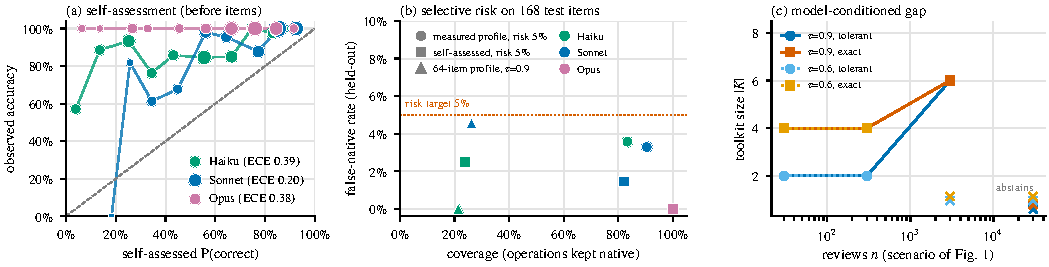
\includegraphics[width=\textwidth]{evaluation_tsc/figures/fig_rq1_profile}
\caption{Model profile: (a) self-assessment reliability, (b) coverage versus false-native rate, (c) toolkit size
versus input size (crosses: abstentions).}
\label{fig:ev-profile}
\end{figure*}

Capability boundaries differ by model and by operation (Table~\ref{tab:ev-calibration}). Haiku fails counting
from $n=40$, Sonnet loses joins as they grow, and both fail approximate sums over 640 values, whereas Opus answers
all 387 items it was given. With the measured profile and a 5\% risk target, the held-out false-native rate stays
within the target for every model (3.6\%, 3.3\% and 0.0\%) while 83--100\% of the operations remain with the model
(Fig.~\ref{fig:ev-profile}b). Both baselines fail. Self-assessment is miscalibrated for every model (ECE
0.20--0.39, all underconfident; Fig.~\ref{fig:ev-profile}a), and the 64-item profile keeps only 21--26\% of the
operations native, sending most correctly performed work to tools. The gap, in turn, behaves as designed
(Fig.~\ref{fig:ev-profile}c): two tools suffice for 30 or 300 reviews and six for 3,000, and the engine abstains
rather than return an unsupported toolkit at 30,000; without gap analysis, it abstains in every setting. On the
test tasks, the profile overrules 9.4\% of the analyst's claims that an operation is native. A measured,
risk-targeted profile therefore makes model conditioning reliable, and neither self-assessment nor a small profile
can replace it.

\subsection{Evidence-Based Eligibility under Forged and Imperfect Metadata}
\label{sec:ev-rq2}

The second experiment addresses RQ2, the restriction of discovery to tools whose safety-relevant behaviour is
evidenced. It measures whether provenance-sound eligibility (P) keeps unsafe tools away from the model, and at what
cost, under a read-only policy over 273 requests with read-only gold tools. Exp@5 is the share of requests whose
top five contain a tool that is not read-only under $J_B$, and Util@5 the share whose top five contain a gold
tool; forgery and verifier errors are simulated. Verified evidence is compared with four encodings of the
policy, namely no filter, MCP's default (annotations displayed, not enforced), annotations as a closed world, and
lexical cues, each combined with \pamcp{}'s retrieval and with MCP-Zero.

\begin{table}[t]
\centering
\caption{Exposure and utility of read-only policy encodings (\%).}
\label{tab:ev-encodings}
\scriptsize
\setlength{\tabcolsep}{2.2pt}
\begin{tabular}{@{}lrrrrrrr@{}}
\toprule
 & & & \multicolumn{2}{c}{\pamcp{} retr.} & \multicolumn{2}{c}{MCP-Zero} & $\delta{=}0.2$ \\
\cmidrule(lr){4-5}\cmidrule(lr){6-7}\cmidrule(l){8-8}
Encoding & Elig. & Unsafe & Exp@5 & Util@5 & Exp@5 & Util@5 & Exp@5 \\
\midrule
no filter & 100.0 & 120 & 42.5 & 49.8 & 26.4 & 76.6 & 43.7 \\
MCP default (display only) & 100.0 & 120 & 42.5 & 49.8 & 26.4 & 76.6 & 43.7 \\
closed-world annotations & 7.7 & 1 & 31.5 & 0.4 & 0.0 & 0.4 & 58.7 \\
lexical cues & 67.8 & 21 & 9.9 & 41.0 & 12.5 & 65.6 & 8.8 \\
verified evidence (P) & 77.0 & 0 & 0.0 & 46.2 & 0.0 & 72.2 & 5.5 \\
observed + lexical fallback & 77.0 & 0 & 0.0 & 46.2 & 0.0 & 72.2 & 5.5 \\
attested only & 26.4 & 0 & 0.0 & 16.5 & 0.0 & 18.3 & 5.8 \\
\bottomrule
\end{tabular}
\end{table}

\begin{figure*}[t]
\centering
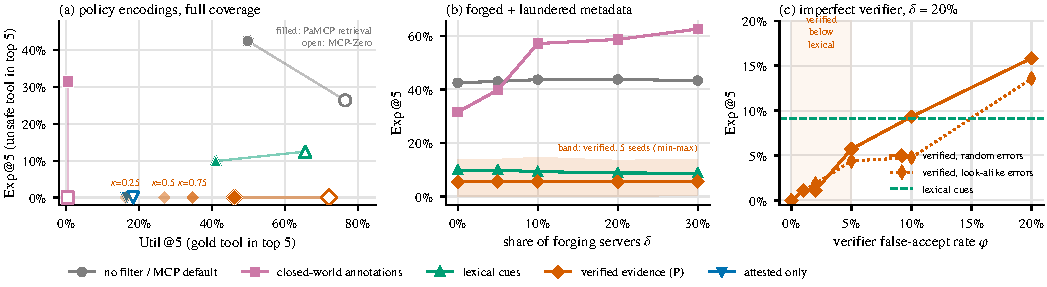
\includegraphics[width=\textwidth]{evaluation_tsc/figures/fig_rq2_exposure}
\caption{Exposure to unsafe tools: (a) policy encodings, (b) forged metadata, (c) verifier false accepts.}
\label{fig:ev-exposure}
\end{figure*}

Every baseline encoding exposes unsafe tools (Table~\ref{tab:ev-encodings}): 42.5\% of the requests without a
filter or under MCP's default, 31.5\% with annotations as a closed world (whose utility falls to 0.4\%), and 9.9\%
with lexical cues. Verified evidence admits none of the 120 unsafe tools, keeps 77\% of the registry eligible and
costs 3.6 utility points (4.4 for MCP-Zero); its difference to lexical cues is confirmatory (F4: $-9.9$ points,
$p_{\mathrm{Holm}}<0.001$). Under forgery, the closed-world reading collapses (31.5\% to 62.6\% exposure at
$\delta=0.3$), while verified evidence stays at 5.4--5.6\% for every $\delta$ with a 5\% false-accept rate
(Fig.~\ref{fig:ev-exposure}b) and remains below lexical cues up to $\varphi=5\%$ (10\% for look-alike errors;
Fig.~\ref{fig:ev-exposure}c).

\begin{figure*}[t]
\centering
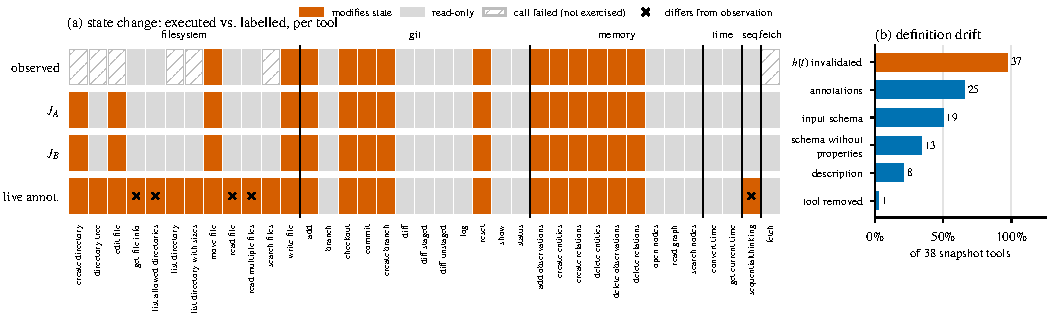
\includegraphics[width=\textwidth]{evaluation_tsc/figures/fig_rq2_observed}
\caption{Executed reference servers: (a) observed and labelled state changes, (b) definition drift since the
benchmark snapshot.}
\label{fig:ev-observed}
\end{figure*}

Three further checks remove the dependency on how the labels were built. First, with the verifier simulated from
$J_B$ and scored on $J_A$, exposure is 2.3--3.9\% across \pamcp{}, RAG-MCP, MCP-Zero and ToolScope, a quarter to
two fifths of the exposure left by lexical cues. Second, when the six MCP reference servers are executed under
system-call tracing (observed; Fig.~\ref{fig:ev-observed}), both labellings agree with all 30 completed calls: none
of the 13 tools observed to change state is labelled read-only (Wilson upper bound 22.8\%). Third, every one of the
37 surviving definitions changed since the benchmark snapshot, so evidence not bound to $h(t)$, as \pamcp{} binds
it, would have been stale. Eligibility based on verified, hash-bound evidence thus removes the exposure that
published metadata leaves, degrades in proportion to verifier error, and does not depend on the reference labels.

\subsection{Compactness and Joint Feasibility of Certified Toolkits}
\label{sec:ev-rq3}

The third experiment addresses RQ3, the return of a small toolkit whose interfaces, effects and flows are
certified jointly before any call. It examines whether set-level reasoning returns smaller toolkits that are
jointly feasible more often than retrieval on the 94 test tasks, against RAG-MCP, COLT and ToolScope (top five),
MCP-Zero, CMTF and per-subtask retrieval, each also restricted to eligible tools. Group recall is measured against
benchmark gold (measured), and joint feasibility is decided by two evaluators written independently of the
certificate: a coarse one, and a strict one that also checks domains, cardinality, schema-required inputs and
egress of private data (labelled). On ten hand-built cases with known answers, the strict evaluator decides 7
correctly and the coarse one 2.

\begin{table}[t]
\centering
\caption{Toolkit size, recall and joint feasibility on the 94 test tasks.}
\label{tab:ev-sets}
\scriptsize
\setlength{\tabcolsep}{2.1pt}
\begin{tabular}{@{}lrrlrrr@{}}
\toprule
 & & & & \multicolumn{2}{c}{Joint feas. (\%)} & \\
\cmidrule(lr){5-6}
Method & $|K|$ & Tok. & Group recall [CI] & coarse & strict & Abst. \\
\midrule
\pamcp{} ($K{=}10$) & 1.46 & 198 & 0.174 [0.12, 0.23] & 67.0 & 27.7 & 7.4 \\
\pamcp{}-L & 1.22 & 146 & 0.161 & 54.7 & 15.8 & 9.5 \\
\pamcp{} NoCert & -- & -- & -- & 59.6 & 13.8 & 0.0 \\
Per-subtask (elig.) & 2.59 & 346 & 0.249 [0.19, 0.32] & 62.8 & 8.5 & -- \\
RAG-MCP@5 (elig.) & 5.00 & 1244 & 0.293 [0.22, 0.37] & 60.6 & 5.3 & -- \\
COLT@5 (elig.) & 5.00 & 1094 & 0.295 [0.23, 0.37] & 59.6 & 8.5 & -- \\
ToolScope@5 (elig.) & 5.20 & 976 & 0.361 [0.29, 0.44] & 73.4 & 11.7 & -- \\
MCP-Zero (elig.) & 1.76 & 250 & 0.227 [0.17, 0.29] & 57.4 & 11.7 & -- \\
CMTF (elig.) & 0.64 & 105 & 0.072 [0.04, 0.11] & 25.5 & 14.9 & -- \\
RAG-MCP@5 (published) & 5.00 & 1244 & 0.293 [0.22, 0.37] & 48.9 & 5.3 & -- \\
\bottomrule
\end{tabular}
\end{table}

\begin{figure*}[t]
\centering
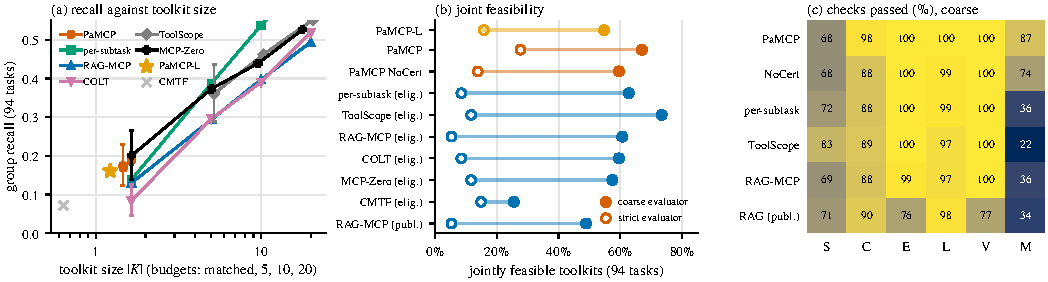
\includegraphics[width=\textwidth]{evaluation_tsc/figures/fig_rq3_sets}
\caption{Toolkit quality: (a) recall versus toolkit size, (b) joint feasibility, (c) certificate checks passed
(S goals, C inputs, E effects, L flows, V evidence, M minimality).}
\label{fig:ev-sets}
\end{figure*}

\pamcp{} returns the smallest toolkits apart from CMTF, with 1.46 tools and 198 tokens against 5 tools and
976--1,244 tokens for the top-five retrievers (Table~\ref{tab:ev-sets}), and it certifies 92.6\% of the tasks,
abstaining with a counterexample on the rest. Under the strict evaluator, its toolkits are jointly feasible in
27.7\% of the tasks, 1.9 to 5.2 times as often as every baseline restricted to eligible tools (5.3--14.9\%) and
twice as often as without certification (13.8\%; Fig.~\ref{fig:ev-sets}b). Certification acts through obtainable
inputs and minimality (C 88\% to 98\%, M 74\% to 87\%, against 22--36\% for the top-five retrievers;
Fig.~\ref{fig:ev-sets}c). At equal size, \pamcp{} reaches more gold steps than RAG-MCP, per-subtask retrieval and
COLT (0.189 against 0.130, 0.138 and 0.084; F2 not significant after correction), whereas retrievers that expose
three to four times more tools reach more (0.249--0.361; non-inferiority to per-subtask retrieval, F1, not shown).
\pamcp{} thus trades breadth for certified compactness.

\begin{table}[t]
\centering
\caption{Single-tool retrieval accuracy on the 300 test requests.}
\label{tab:ev-retrieval}
\scriptsize
\setlength{\tabcolsep}{2.4pt}
\begin{tabular}{@{}lrrrrrr@{}}
\toprule
 & 81 tools & \multicolumn{5}{c}{569 tools} \\
\cmidrule(lr){2-2}\cmidrule(l){3-7}
Method & Hit@1 & Hit@1 [CI] & Hit@3 & Hit@5 & MRR & nDCG \\
\midrule
BM25 & 52.7 & 41.0 [26, 60] & 57.3 & 63.7 & 0.503 & 0.543 \\
RAG-MCP (dense) & 49.7 & 37.3 [22, 56] & 50.0 & 54.3 & 0.451 & 0.492 \\
RRF fusion & 54.3 & 38.7 [23, 57] & 54.7 & 61.3 & 0.481 & 0.525 \\
MCP-Zero & 68.0 & 66.7 [49, 80] & 80.0 & 85.7 & 0.743 & 0.775 \\
COLT & 49.7 & 37.3 [22, 56] & 50.0 & 54.3 & 0.451 & 0.492 \\
ToolScope & 53.0 & 41.0 [26, 60] & 58.3 & 63.7 & 0.504 & 0.543 \\
CMTF & 58.7 & 32.7 [19, 49] & 47.0 & 54.7 & 0.428 & 0.488 \\
PaMCP (Eq. 5) & 61.0 & 29.7 [16, 47] & 45.7 & 53.7 & 0.400 & 0.461 \\
PaMCP-L & 72.0 & 41.3 [25, 60] & 61.3 & 69.3 & 0.536 & 0.603 \\
PaMCP, oracle types (diag.) & 71.7 & 58.3 [38, 74] & 75.3 & 81.3 & 0.680 & 0.728 \\
\bottomrule
\end{tabular}
\end{table}

Single-tool retrieval, in contrast, is not where \pamcp{} gains (Table~\ref{tab:ev-retrieval}). Over 81 tools, its
relevance-first ranking is the most accurate (72.0\% Hit@1, against 68.0\% for MCP-Zero), but over the full
registry MCP-Zero leads (66.7\%), \pamcp{}-L ties tuned BM25 (41.3\% against 41.0\%; H1 n.s.), and the structural
ranking of Eq.~(5) falls to 29.7\% (F7 against \pamcp{}), because types agree with $J_B$ on 78.9\% of output kinds
but only on 35.7\% of domains. With correct types, the same ranking reaches 58.3\%, above every baseline except
MCP-Zero, which locates the limit in the typing rather than in the composition. Set-level reasoning therefore
yields the most compact and most often jointly feasible toolkits, while finding more tools requires better typing
or a larger budget.

\subsection{Resistance to Injected Actions and Contribution of the Mechanisms}
\label{sec:ev-sec}

The fourth experiment combines RQ2 and RQ3. It measures whether the exposed
toolkit limits what an injected instruction could achieve, and which mechanism is responsible. For 155 tasks and
each attack class outside the task's needs, an attack is reachable if the toolkit can realise it under $J_B$
(labelled, offline). Poisoning places a canary in the description, name or argument keys of 10--30\% of the tools,
and we scan what each method shows the model; the mechanisms are varied in a $2^3$ design with Shapley
attribution.

\begin{figure*}[t]
\centering
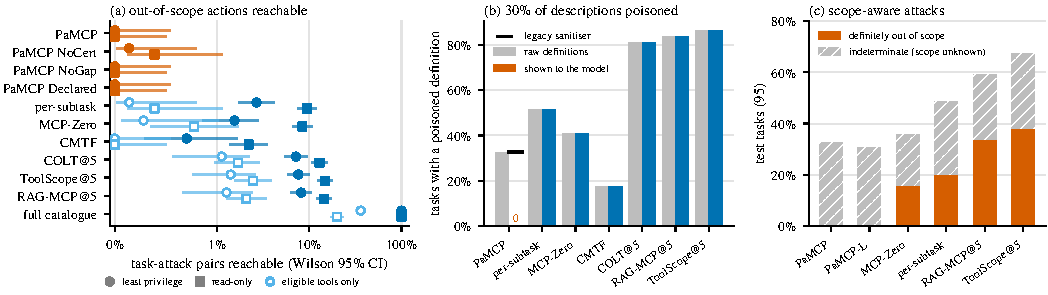
\includegraphics[width=\textwidth]{evaluation_tsc/figures/fig_sec_injection}
\caption{Injected actions: (a) reachable out-of-scope actions, (b) poisoned definitions shown to the model,
(c) scope of admitted attacks.}
\label{fig:ev-injection}
\end{figure*}

No out-of-scope action is reachable through \pamcp{}'s toolkits: 0 of 712 task--attack pairs under least privilege
and 0 of 775 under a read-only policy, against 0.7--8.1\% and 8.4--14.7\% for the published baselines
(Fig.~\ref{fig:ev-injection}a; F5, $p_{\mathrm{Holm}}<0.001$). Counting only attacks that are definitely out of
scope, no \pamcp{} toolkit admits one, against 15.8\% of the tasks for MCP-Zero, 20.0\% for per-subtask retrieval,
33.7\% for RAG-MCP and 37.9\% for ToolScope (H5: $-20.0$ points, 95\% CI $[-28.4,-12.6]$,
$p_{\mathrm{Holm}}<0.001$), although 32.6\% admit an attack whose scope the labels cannot decide. With 30\% of the
descriptions poisoned, the aliased manifest never shows an injected instruction, whereas the definitions exposed
by the baselines carry one in 17.4--86.2\% of the tasks (Fig.~\ref{fig:ev-injection}b). Moreover, 55.5\% of
\pamcp{}'s toolkits return remote content, but none of them also enables an out-of-scope action, against
3.2--22.6\% for the baselines.

\begin{table}[t]
\centering
\caption{Ablation of the gap (G), eligibility (P) and set reasoning (S).}
\label{tab:ev-factorial}
\scriptsize
\setlength{\tabcolsep}{3pt}
\begin{tabular}{@{}cccrrrrr@{}}
\toprule
G & P & S & Recall & Tokens & Joint (\%) & Reach (\%) & Abst. (\%) \\
\midrule
-- & -- & -- & 0.270 & 297 & 53.5 & 1.1 & 0.0 \\
on & -- & -- & 0.239 & 208 & 55.5 & 0.4 & 0.0 \\
-- & on & -- & 0.295 & 316 & 58.1 & 0.1 & 0.0 \\
-- & -- & on & 0.223 & 221 & 52.9 & 0.1 & 16.1 \\
on & on & -- & 0.253 & 229 & 56.8 & 0.1 & 0.0 \\
on & -- & on & 0.230 & 189 & 54.8 & 0.0 & 6.5 \\
-- & on & on & 0.183 & 193 & 55.5 & 0.0 & 20.0 \\
on & on & on & 0.181 & 176 & 56.1 & 0.0 & 10.3 \\
\midrule
\multicolumn{3}{@{}l}{Full, no backward closure} & 0.181 & 173 & 53.5 & 0.0 & 12.3 \\
\multicolumn{3}{@{}l}{Full, flow along derivations} & 0.236 & 206 & 60.6 & 0.0 & 5.8 \\
\multicolumn{3}{@{}l}{Full, no relevance term} & 0.167 & 141 & 54.8 & 0.0 & 10.3 \\
\multicolumn{3}{@{}l}{Full, no utility floor} & 0.181 & 176 & 56.1 & 0.0 & 10.3 \\
\multicolumn{3}{@{}l}{Full, no refinement} & 0.179 & 175 & 55.5 & 0.0 & 11.0 \\
\bottomrule
\end{tabular}
\end{table}

The factorial design (Table~\ref{tab:ev-factorial}) shows that each mechanism contributes. Eligibility removes
most reachable actions, and with gap analysis and set reasoning, reachability falls from 5.2\% of the tasks to none
(Shapley shares of 23\%, 35\% and 42\% for G, P and S). Gap analysis and set reasoning shrink the context from 297
to 176 tokens (main effects of $-56$ and $-67$ tokens, $p<0.001$), and the gap halves abstentions (10.3\% against
20.0\%). The price is recall (0.270 to 0.181, mainly through S), and no mechanism changes the coarse joint
feasibility. Under the labelled threat model, \pamcp{}'s mechanisms therefore jointly close the action and
metadata channels that retrieval baselines leave open.

\subsection{Scalability, Optimality and Adaptation to Registry Change}
\label{sec:ev-eff}

The last experiment addresses RQ4, discovery at a cost that scales and under registry change, together with the
optimality of the composition studied under RQ3. It measures what discovery costs, how close the composition is
to the optimum, and whether the engine keeps its guarantees under change. The engine is compared with eager
materialisation of the risk relation, with the greedy regime and an integer program (HiGHS) written independently
of the engine, with full rebuilds and cache flushes, and with cold discovery without experience reuse.

\begin{figure*}[t]
\centering
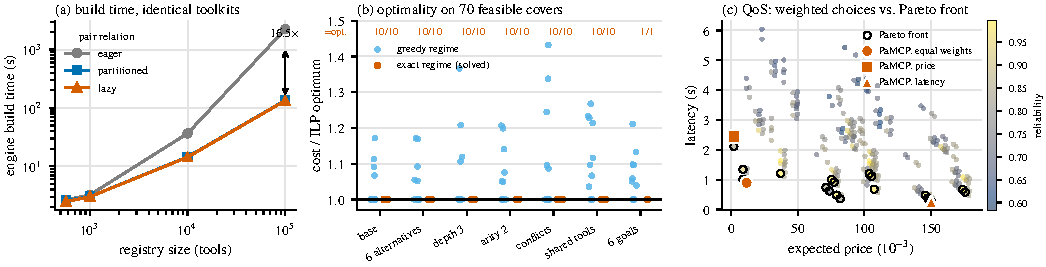
\includegraphics[width=\textwidth]{evaluation_tsc/figures/fig_tsc_eff}
\caption{Efficiency: (a) engine build time by pair-relation mode, (b) cost relative to the ILP optimum, (c) QoS
choices and Pareto front.}
\label{fig:ev-eff}
\end{figure*}

On the real registry, a request takes 49\,ms at the median (eligibility 0.08\,ms, against 12\,ms for RAG-MCP's
single dense ranking) and 2.7\,s at $10^5$ cloned tools. Deciding the pairwise risk relation lazily or by effect
class gives identical toolkits on all test tasks and builds the engine at $10^5$ tools in 133--134\,s instead of
2,224\,s, 16.5 times faster with near-linear growth (Fig.~\ref{fig:ev-eff}a); on heterogeneous registries of
$10^4$ tools, the lazy build takes 4.6--5.9\,s. Wherever the exact search finishes, it returns the ILP optimum (61
of 61 solved instances across alternatives, depth, arity, conflicts and shared tools) and recognises all ten
infeasible instances, while the greedy regime is 4.4--12.6\% above the optimum on average
(Fig.~\ref{fig:ev-eff}b); with six goals, the search exhausts its budget and falls back to greedy (6.9\% above).
When providers differ in price, latency and reliability, every equal-weight choice is Pareto-optimal and meets the
utility floor, and the weights move the choice along the front as intended (price only: 0.33$\times$ price;
latency only: 0.73$\times$ latency; Fig.~\ref{fig:ev-eff}c).

The engine also adapts to change at low cost. An incremental update takes 13.5\,ms against 4.2\,s for a rebuild,
the exact invalidation of Proposition~3 touches 1.1\% of the cached toolkits instead of all of them, and all 20
simulated rug pulls lose their evidence. Experience reuse serves 32.7\% of 300 requests without an analyst call,
with unchanged certification (82.7\% against 82.3\%) and no violation in 89 revalidation probes (removed servers,
revoked or rewritten tools, stricter principal, other model). Deterministic repair raises certification from
72.6\% to 87.4\% when counterexamples are induced. The complete engine thus scales to $10^5$ tools, composes
optimally where it searches exactly, makes Pareto-consistent QoS trade-offs and adapts to change without losing
its guarantees.

\subsection{Summary of Findings and Threats to Validity}
\label{sec:ev-threats}

\begin{table}[t]
\centering
\caption{Summary of findings (Conf.: confirmatory test, $p_{\mathrm{Holm}}$).}
\label{tab:ev-answers}
\scriptsize
\setlength{\tabcolsep}{2pt}
\begin{tabular}{@{}lp{2.85cm}p{2.95cm}l@{}}
\toprule
Aspect & Result & Best baseline & Conf. \\
\midrule
Profile & FNR $\le$3.6\% at 83--100\% coverage & self-assessment ECE 0.20--0.39 & -- \\
Eligibility & Exp@5 0\% (swap 2.3--3.9\%), Util $-3.6$ & lexical 9.9\%, MCP default 42.5\% & F4 $<$0.001 \\
Execution & labels = execution, 30/30 calls & -- (observed) & -- \\
Feasibility & strict joint 27.7\%, 1.46 tools & 5.3--14.9\%, 0.64--5.2 tools & expl. \\
Recall & recall at equal size 0.189 & 0.084--0.200 & F2 n.s. \\
Retrieval & Hit@1 (569) 41.3\% & MCP-Zero 66.7\% & F7 against \\
Security & reachable 0/712, definite 0\% & 0.7--8.1\%, 15.8--37.9\% & F5, H5 $<$0.001 \\
Scaling & build 16.5$\times$ faster; =ILP 61/61 & eager 2,224\,s; greedy +4--13\% & -- \\
Evolution & update 13.5\,ms; reuse 32.7\% & rebuild 4.2\,s; cold & -- \\
\bottomrule
\end{tabular}
\end{table}

\begin{table}[t]
\centering
\caption{Confirmatory comparisons (Holm-corrected; $\Delta$: \pamcp{} minus comparator, in points, tokens for F6).}
\label{tab:ev-family}
\scriptsize
\setlength{\tabcolsep}{2.2pt}
\begin{tabular}{@{}llrlll@{}}
\toprule
 & Comparison & $\Delta$ & 95\% CI & $p_{\mathrm{Holm}}$ & Verdict \\
\midrule
F1 & Group recall vs per-subtask (non-inf., 0.05) & -8.0 & [-16.6, +0.2] & 1.000 & not shown \\
F2 & Size-matched recall vs RAG-MCP & +6.0 & [-1.6, +13.7] & 0.397 & n.s. \\
F3 & Joint feasibility vs per-subtask (elig.) & +4.3 & [-8.5, +18.1] & 1.000 & n.s. \\
F4 & Exp@5 verified vs lexical & -9.9 & [-13.9, -6.6] & $<$0.001 & supports \\
F5 & Reachable attacks vs per-subtask & -2.7 & [-3.9, -1.5] & $<$0.001 & supports \\
F6 & Tokens, full vs NoGap & -16.7 & [-34.6, +1.0] & 0.269 & n.s. \\
F7 & Hit@1 goal contract vs raw RRF (569) & -15.7 & [-21.3, -10.0] & $<$0.001 & against \\
\midrule
H1 & Hit@1 PaMCP-L vs tuned BM25 (569) & +0.3 & [-8.9, +8.8] & 1.000 & n.s. \\
H2 & Hit@1 PaMCP-L vs Eq. (5) (569) & +11.7 & [+3.0, +22.6] & 0.070 & n.s. \\
H3 & Group recall PaMCP-L vs per-subtask (non-inf.) & -8.8 & [-17.6, -0.5] & 1.000 & not shown \\
H4 & Strict joint feas. vs per-subtask (elig.) & +7.4 & [+0.0, +14.9] & 0.277 & n.s. \\
H5 & Definite out-of-scope vs per-subtask & -20.0 & [-28.4, -12.6] & $<$0.001 & supports \\
\bottomrule
\end{tabular}
\end{table}

Table~\ref{tab:ev-answers} summarises the findings for RQ1--RQ4, and Table~\ref{tab:ev-family} the confirmatory
tests. All confirmatory tests on safety (F4, F5 and H5) favour \pamcp{} at $p_{\mathrm{Holm}}<0.001$; the tests on
recall and retrieval do not, and the feasibility advantage under the strict evaluator is exploratory.

These findings are subject to several threats to validity. Effects, types and feasibility are scored against LLM
labels; execution confirms them on 30 calls of six non-adversarial reference servers, and the label swap bounds
the effect of labeller disagreement but not of errors shared by one model family. Reachability is decided offline:
whether an agent follows an injected instruction, and end-to-end task success, require executing the toolkits,
which this study did not do. The baselines are adaptations sharing a TF-IDF and SVD encoder, all tuned on the same
development split; larger registries are cloned or generated, and QoS data are synthetic. Executed compositions
over isolated and adversarial servers, human annotation of a stratified tool sample and reproductions of the
baselines with their original encoders are the natural next steps, and the released artifact supports each of
them.
